%-------------------------------------------------------------------------------
%                            BAB IV
%               		HASIL DAN PEMBAHASAN
%-------------------------------------------------------------------------------

\chapter{HASIL DAN PEMBAHASAN}
	\section{Pengumpulan Data}
	
	%\begin{table}[H]
	%	\centering
	%	\caption{Jadwal Penelitian.}
	%	\label{jadwal}
	%	\begin{tabular}{|p{10cm}|}
	%		\hline
	%		Context Admin :: nonAktifKos(idKos:int)\\ 
	%		pre: kjdksnckls \\ \hline
	%	\end{tabular}
	%\end{table}

	Tahap pertama yang dilakukan pada penelitian ini adalah mengumpulkan data dengan cara observasi dan wawancara. Data yang didapat digunakan untuk membangun aplikasi pencarian dan pemesanan kos-kosan ini. Berikut penjelasan dari setiap tahap pengumpulan data.
	
	\subsection{Observasi}
	Pada saat observasi, yang dilakukan di Banda Aceh dan sekitarnya, hal yang diperhatikan adalah media iklan yang dilakukan pemilik kos untuk mempromosikan kosnya dan apa saja isi dari iklan tersebut.  Setelah melakukan pengamatan, hasil yang didapat adalah banyaknya spanduk, brosur dan sejenisnya yang tersebar di daerah kampus seperti Universitas Syiah Kuala, UIN Ar-raniry, Universitas Muhammadyah dan lain-lain. Media iklan tersebut banyak ditemui di mading, di pohon, di dinding dan tempat dimana mahasiswa beraktifitas. Selain di kampus, promosi kos juga terdapat di persimpangan jalan atau di perempatan lampu merah. Isi dari iklan kos-kosan beragam, mulai dari memuat informasi yang lengkap, hingga informasi yang tertera hanya alamat dan nomor yang dapat dihubungi. 
	
	\subsection{Wawancara}
	Sebelum memulai wawancara, hal yang dilakukan adalah menentukan kelompok \textit{user} (pengguna) terlebih dahulu. Kelompok yang ditentukan adalah pemilik kos, anak kos dan admin tetapi kelompok pengguna admin tidak diwawancarai. Setelah menentukan kelompok pengguna, selanjutnya adalah menentukan pertanyaan-pertanyaan yang akan ditujukan kepada pengguna dan menentukan berapa orang yang akan diwawancarai. Pertanyaan untuk pemilik kos dan anak kos sekitar 10 pertanyaan seputar promosi kos-kosan dan pencarian kos-kosan dan jumlah orang yang diwawancarai adalah 10 orang/kelompok pengguna. Wawancara pemilik kos dan anak kos dilakukan dengan cara mengunjungi langsung kos-kosan yang ada di Banda Aceh dan sekitarnya. 
	
	Berdasarkan wawancara, pemilik kos mempromosikan kosnya dengan cara menempelkan brosur, pamplet, spanduk atau sejenisnya disekitar kampus dan menempelkan papan informasi di depan kosnya bahwa menerima anak kos. Kendala yang dihadapi dalam usaha kos-kosan adalah ketika bukan pada masa ajaran baru, sulit untuk mendapatkan anak kos. Oleh karena itu terkadang pemilik kos tidak memberikan jangka waktu yang hanya beberapa bulan untuk menyewa kos, kecuali selesai menyewa pada saat mendekati ajaran baru. Selain itu, para pemilik kos yang menyebarkan informasi kosannya harus mengingat dimana letak promosi tersebut karena jika kamar kos sudah penuh, iklan tersebut akan dicabut, hal ini dilakukan untuk mengurangi telepon dari pencari kos.
	
	Berdasarkan wawancara anak kos, pada saat menjadi mahasiswa baru mereka mencari kos dengan cara melihat iklan kos-kosan disekitar kampus maupun berkeliling disekitar kampus. Pada iklan kosan memuat alamat dan nomor yang dapat dihubungi, sehingga mereka akan menuju ke lokasi kos atau menghubungi pemilik kos terlebih dahulu. Pencari kos yang mendatangi langsung kos akan melihat kondisi rumah dan fasilitas kos, jika kebetulan pemilik kos berada ditempat, pencari kos akan menanyakan seputar kos dan kamar yang kosong. Namun, jika pemilik kos tidak ditempat, pencari kos akan menghubungi pemilik kos. Ketika pencari kos tertarik dan pemilik kos setuju, maka terjadi transaksi dan pemilik kos dapat menyewa kamar tersebut. Jika pencari kos merasa kurang cocok, mereka akan mencari ke tempat kos lain.
	
	\section{Perencanaan Sistem}
	Aplikasi yang dibangun ditujukan kepada pemilik kos, pencari kos dan admin. Aplikasi berbasis web digunakan pemilik kos dan admin. Pemilik kos dapat mempromosikan kos miliknya, sedangkan admin bertugas untuk memantau  dan memverifikasi data kos-kosan yang terdaftar untuk menghindari kepalsuan data. Aplikasi Android digunakan oleh pencari kos. 
	
	Aplikasi ini dirancang berdasarkan masalah atau \textit{problem-based analysis} dengan menggunakan \textit{problem frames}. Untuk mencapai \textit{problem frames}, tahap yang dilakukan terdiri dari membuat \textit{user stories}, \textit{requirement}, menentukan domain dan \textit{share phenomena}. 
	
	\subsection{\textit{User Stories}}
	Tahap pertama adalah menentukan masalah dengan membuat \textit{user stories}. \textit{User stories} dibuat berdasarkan wawancara yang telah dilakukan sebelumnya. \textit{User stories} ditulis dengan format "\textbf{sebagai <tipe pengguna>, saya ingin <melakukan tindakan tertentu atau mendapatkan suatu fungsi tertentu> sehingga <mendapatkan manfaat atau nilai bisnis tertentu>}". \textit{User stories }terbagi menjadi 3 bagian, yaitu pemilik kos, pencari kos serta admin. Berikut adalah daftar \textbf{user stories}:

		\begin{enumerate}[a.]
		
			\item Pencari Kos
			
				\begin{itemize}
					\item Sebagai pencari kos, saya ingin melihat semua daftar kos-kosan sehingga saya dapat memilih kos untuk ditempati.
					\item Sebagai pencari kos, saya ingin memilih kos berdasarkan wilayah/ daerah sehingga saya dapat menemukan kos di daerah yang diinginkan.
					\item Sebagai pencari kos, saya ingin memilih kos berdasarkan jenis kos, rentang harga maupun fasilitas sehingga saya dapat menemukan kos idaman dengan mudah.
					\item Sebagai pencari kos, saya ingin melihat detail informasi dari kos seperti harga, fasilitas, alamat lengkap, dll sehingga saya tidak perlu bertanya lagi kepada pemilik kos.
					\item Sebagai pencari kos, saya ingin petunjuk arah kos sehingga saya tidak tersesat ketika mencari kos.
					\item Sebagai pencari kos, saya ingin memesan kos sehingga tidak takut kehabisan kamar kos.
					\item Sebagai pencari kos, saya ingin melihat riwayat kos yang pernah saya tinggali sehingga saya mengetahui kos yang pernah ditinggali.
					\item Sebagai pencari kos, saya ingin membatalkan pesanan kos jika saya salah input sehingga pemilik kos tidak perlu menghubungi saya.
					\item Sebagai pencari kos, saya ingin memberikan penilaian terhadap kos yang pernah saya tinggali sehingga dapat memberikan kritik atau saran yang membangun kepada pemilik kos.
				\end{itemize}
			
			\item Pemilik Kos
			
			\begin{itemize}
				\item Sebagai pemilik kos, saya ingin mempromosikan kos saya kepada orang-orang yang mencari kos sehingga saya tidak perlu melakukan iklan dengan brosur dan lain-lain lagi.
				\item Sebagai pemilik kos, saya ingin mengisi data kos dan kamar sehingga dapat dipromosikan.
				\item Sebagai pemilik kos, saya ingin memberikan petunjuk arah kos sehingga pencari kos tidak kebingungan mencari kos saya.
				\item Sebagai pemilik kos, saya ingin melihat daftar orang-orang yang memesan kos saya sehingga bisa saya pilih untuk menjadi anak kos.
				\item Sebagai pemilik kos, saya ingin memilih atau menyetujui orang-orang yang memesan kos saya sehingga tidak sembarangan orang yang dapat menyewa kos saya.
				\item Sebagai pemilik kos, saya ingin memasukkan tanggal masuk dan tanggal keluar penyewa kos sehingga saya bisa melihatnya kembali jika saya lupa.
				\item Sebagai pemilik kos, saya ingin melihat daftar penyewa yang ada di kos saya sehingga saya bisa memiliki data penyewa kos.
				\item Sebagai pemilik kos, saya ingin melihat daftar penilaian dari pencari kos, sehingga kos saya dapat menjadi lebih baik lagi.
			\end{itemize}
		
		\item Admin
		\begin{itemize}
			\item Sebagai admin, saya ingin melihat seluruh data pemilik kos sehingga saya dapat mengetahui pemilik kos yang mendaftar
			\item Sebagai admin, saya ingin melihat seluruh data kos sehingga saya dapat survey langsung kos tersebut.
			\item Sebagai admin, saya ingin memverifikasi kos sehingga kos yang akan tampil pada aplikasi adalah kos dengan data yang sebenarnya.
			\item Sebagai admin, saya ingin menambahkan fasilitas kos, fasilitas kamar dan akses sekitar sehingga jika ada data yang belum di-input, dapat di-input.
			\item Sebagai admin, saya ingin melihat daftar pencari kos yang memesan kos sehingga saya dapat mengetahui siapa memesan kos apa.
			\item Sebagai admin, saya ingin melihat daftar penyewa kos sehingga saya dapat mengetahui siapa menyewa kos apa.
			\item Sebagai admin, saya ingin melihat daftar penilaian penyewa kos terhadap kos sehingga saya dapat mengetahui penilaian baik dan buruk kos dan dapat melakukan evaluasi terhadap kos.
			\item Sebagai admin, saya ingin dapat menonaktifkan atau aktifkan akun atau kos jika terdapat kesalahan atau permintaan dari pemilik kos.
		\end{itemize}
			
		\end{enumerate}
	\subsection{\textit{Requirement} dan \textit{Domain Knowledge }}
	Berdasarkan \textit{user stories} tersebut, dikembangkan menjadi \textit{requirement} kemudian menentukan \textit{domain knowledge} dan \textit{share phenomena}. Berikut adalah \textit{requirement} ditulis dengan format R[nomor]:
	\begin{enumerate} [a.]
		\item Pencari Kos
		
		R01. Pencari kos dapat melihat semua informasi kos \\
		R02. Pencari kos dapat mencari informasi kos berdasarkan wilayah \\
		R03. Pencari kos dapat mencari informasi kos berdasarkan tipe kos \\
		R04. Pencari kos dapat mencari informasi kos berdasarkan fasilitas kos \\
		R05. Pencari kos dapat mencari informasi kos berdasarkan harga terendah-tertinggi \\
		R06. Pencari kos dapat mencari informasi kos berdasarkan harga tertinggi-terendah \\
		R07. Pencari kos dapat mencari informasi kos berdasarkan nama kos \\
		R08. Pencari kos dapat melihat informasi detail tentang kos \\
		R09. Pencari kos dapat mengetahui petunjuk lokasi kos \\
		R10. Pencari kos dapat memesan kamar kos dengan memasukkan data diri \\
		R11. Pencari kos dapat melihat riwayat pemesanan kos \\
		R12. Pencari kos dapat melihat kos yang sedang ditempati \\
		R13. Pencari kos dapat membatalkan pesanan \\
		R14. Pencari kos dapat memberikan penilaian terhadap kos \\
		R15. Pencari kos dapat memindai QR Code untuk mengetahui informasi suatu kos \\
		
		\item Pemilik Kos
		
		R16. Pemilik kos dapat memasukkan data kos untuk dipromosikan \\
		R17. Pemilik kos dapat mengedit data kos \\
		R18. Pemilik kos dapat memberikan petunjuk arah menuju kosnya \\
		R19. Pemilik kos dapat memilih atau menyetujui orang-orang yang memesan kos \\
		R20. Pemilik kos dapat memasukkan tanggal masuk dan tanggal keluar penyewa kos \\
		R21. Pemilik kos dapat melihat daftar penyewa yang ada di kos \\
		R22. Pemilik kos dapat melihat daftar penilaian dari penyewa kos \\
		R23. Pemilik kos dapat mengunduh QR Code yang berisi informasi tentang kos \\
		
		\item Admin
		
		R24. Admin dapat melihat semua data pemilik kos yang mendaftar \\
		R25. Admin dapat melihat semua data kos \\
		R26. Admin dapat mengnon-aktifkan/mengaktifkan kos dan akun pemilik \\
		R27. Admin dapat memverifikasikan / membatalkan verifikasi kos \\
		R28. Admin dapat menyediakan QR Code yang berisi data suatu kos \\
		R29. Admin dapat menambahkan fasilitas kos, fasilitas kamar dan akses sekitar \\
		R30. Admin dapat melihat daftar pencari kos yang memesan kos \\
		R31. Admin dapat melihat daftar penyewa kos \\ 
		R32. Admin dapat melihat daftar penilaian penyewa kos terhadap kos \\
		
	\end{enumerate}
		\textit{Domain knowledge} yang ditentukan adalah sebagai berikut:
		
		\begin{enumerate}[a.]
			\item \textit{Display} kos memiliki domain Display (D)
			\item \textit{Database} kos memiliki domain \textit{Lexical} (X)
			\item Pengguna memiliki domain Bidable (B)
			\item \textit{Scanner QR Code} memiliki domain Causal (C)
			\item \textit{Generator QR Code} memiliki domain Causal (C)
			\item \textit{Tracking} memiliki domain Causal (C)
		\end{enumerate}
		
		\subsection{\textit{Problem Frames}}
		Setelah menentukan domain, selanjutnya adalah menggambarkan permasalahan dengan menggunakan \textit{problem frames}. Berikut adalah \textit{problem frames} dan penjelasannya bersama \textit{share phenomena}:
		
		\begin{enumerate}[-]
			\item \textit{Model Display} untuk menampilkan data
			
			\textit{Problem frames} yang pertama adalah \textit{Model Display}. Domain pada \textit{model display} adalah \textit{Display} (D) dan \textit{Lexical} (X) dengan domain \textit{Display} yang di-\textit{constrained}. \textit{Frame} ini menggambarkan bahwa aplikasi akan menampilkan data ke \textit{display}. Gambar \ref{pb1} adalah \textit{frame diagram} bernama \textit{model display}.
			
			\begin{figure}[H]
				\centering
				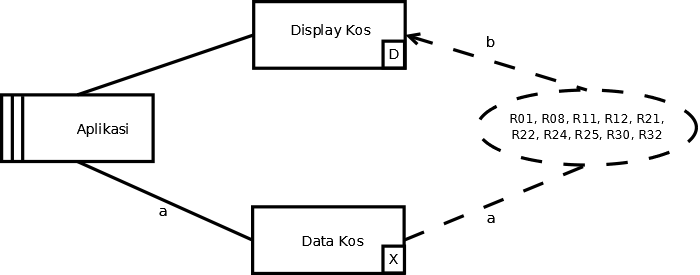
\includegraphics[scale=0.4]{gambar/1}
				\caption{\textit{Frame diagram}: \textit{Model Display}}
				\label{pb1}
			\end{figure}
			
			Berikut adalah penjelasan mengenai \textit{frame} yang berisi domain dan \textit{share phenomena}.
			
			\begin{enumerate}[a.]
				\item App ! ambil-data-kos
				
				DK ! data-kos-diambil
								
				\item D ! tampilkan-data-kos
			\end{enumerate}
		
			App singkatan dari Aplikasi, dapat mengambil data kos. DK singkatan dari Data Kos, yaitu data kos dapat diambil dari \textit{database}. Sedangkan D singkatan dari Display, mengontrol data kos yang akan ditampilkan pada aplikasi. Garis putus-putus menunjukan \textit{requirement}. Sehingga maksud dari gambar \ref{pb1} adalah Aplikasi mengambil data di Data Kos kemudian menampilkannya di Display Kos.
				
			\item \textit{Query}
			
			\textit{Frame diagram Query} menggambarkan aplikasi dimana pengguna dapat melihat data dari \textit{database }tanpa mengubah data tersebut (harus melibatkan pengguna). Domain pada \textit{frame diagram} ini adalah \textit{Lexical} (X), \textit{Display} (D) dan \textit{Bidabble} (B) dengan domain \textit{Display} yang di-\textit{constrained}. Gambar \ref{pb2} adalah \textit{frame diagram query} untuk pengguna dapat melihat data kos.
			
			\begin{figure}[H]
				\centering
				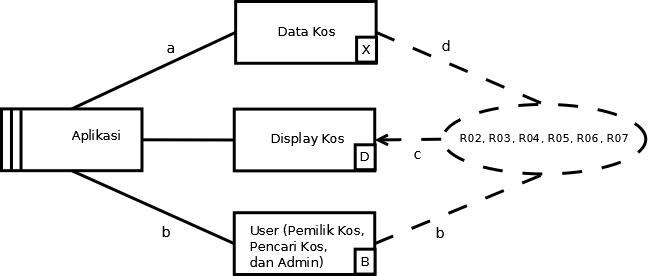
\includegraphics[scale=0.4]{gambar/2}
				\caption{\textit{Frame diagram}: \textit{Query}}
				\label{pb2}
			\end{figure}
		
			Berikut adalah penjelasan dari gambar \ref{pb2}.
			
			\begin{enumerate}[a.]
				\item App ! ambil-data-kos
				
				DK ! data-kos-diambil
				
				\item U ! \textit{input}-pencarian
				\item D ! tampilkan-data-kos
				\item DK ! mencari-data-kos
			\end{enumerate}
		
		Artinya adalah Aplikasi dapat mengambil data kos melalui Data Kos berdasarkan pencarian Pengguna kemudian akan menampilkannya di Display Kos.
		
			\item \textit{Update}
			
			\textit{Frame diagram update} menggambarkan aplikasi dimana pengguna dapat mengubah dan menambahkan data kos. Domain pada \textit{frame diagram} ini adalah \textit{Lexical} (X), \textit{Display} (D) dan \textit{Bidabble} (B) dengan domain \textit{Lexical} dan \textit{Display} yang di-\textit{constrained}. Gambar \ref{pb4} adalah \textit{frame diagram update}.
			
			\begin{figure}[H]
				\centering
				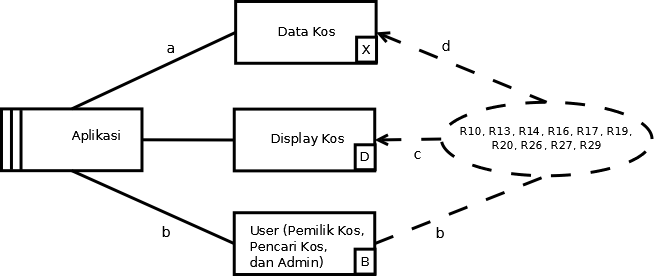
\includegraphics[scale=0.4]{gambar/Update}
				\caption{\textit{Frame diagram: Update}}
				\label{pb4}
			\end{figure}
		
			Berikut adalah penjelasan dari gambar \ref{pb4}.
			
			\begin{enumerate}[a.]
				\item App ! ambil-data-kos
				
				DK ! data-kos-diambil
				
				\item U ! memasukkan-data-kos
				
				U ! mengubah-data-kos
				
				\item D ! tampilkan-data-kos
				\item DK ! menyimpan-data-kos
			\end{enumerate}
		
		Artinya adalah Aplikasi dapat menambah atau mengubah data di Data Kos berdasarkan \textit{input} dari Pengguna, kemudian ditampilkan di Display Kos.
		
			\item \textit{Information + Model Display} untuk mengetahui lokasi kos
			
			\textit{Frame diagram} ini menggambarkan aplikasi yang dapat menampilkan informasi dari alat atau mesin. Domain \textit{frame diagram} ini adalah \textit{Causal} (C), \textit{Display} (D) dan \textit{Lexical} (X) dengan domain \textit{Display} yang di-\textit{constrained}. Gambar \ref{pb5} adalah \textit{frame diagram information+model display} untuk mengetahui lokasi kos.
			
			\begin{figure}[H]
				\centering
				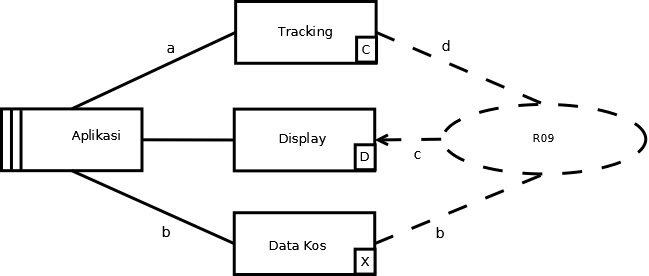
\includegraphics[scale=0.4]{gambar/5}
				\caption{\textit{Frame diagram: Information + Model Display}}
				\label{pb5}
			\end{figure}
			
			Berikut adalah penjelasan dari gambar \ref{pb5}.
			
			\begin{enumerate}[a.]
				\item App ! menyiapkan-peta
				
				T ! peta-disiapkan
				
				\item DK ! mengambil-koordinat-kos
				
				\item D ! tampilkan-lokasi-kos
				\item T ! menerima-koordinat-kos
			\end{enumerate}
		
		Artinya adalah Aplikasi menyiapkan peta dimana akan ditampilkan di Display Kos dengan koordinat kos yang didapat dari Data Kos.
		
			\item \textit{Information + Model Display} untuk membuat \textit{QR Code}
			
			\textit{Frame diagram} untuk membuat \textit{QR Code} menggunakan \textit{frame diagram} yang sama dengan yang sebelumnya, yang membedakan hanya domain dan \textit{share phenomena}. Gambar \ref{pb6} adalah \textit{frame diagram} untuk membuat \textit{QR Code}.
			
			\begin{figure}[H]
				\centering
				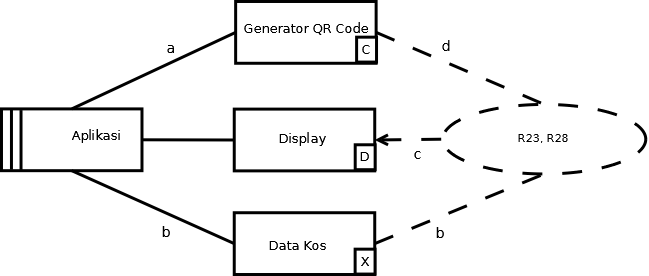
\includegraphics[scale=0.4]{gambar/6}
				\caption{Tampilan halaman ubah password}
				\label{pb6}
			\end{figure}
		
			Berikut adalah penjelasan dari gambar \ref{pb6}.
			
			\begin{enumerate}[a.]
				\item App ! menyiapkan-\textit{generator}
				
				GQC ! \textit{generator}-disiapkan
				
				\item DK ! mengambil-data-kos
				
				\item D ! tampilkan-\textit{qrcode}-kos
				\item GQC ! membuat-\textit{qrcode}-dari-data-kos
			\end{enumerate}
		
		Artinya adalah Aplikasi menyiapkan \textit{generator QR Code} untuk membuat \textit{QR Code} berdasarkan data yang ada pada Data Kos. \textit{QR Code} kemudian dapat ditampilkan di Display Kos.
		
			\item \textit{Information + Model Display} untuk membaca \textit{QR Code}
			
			Gambar \ref{pb7} menggambarkan \textit{frame diagram }yang digunakan untuk membaca \textit{QR Code.}
			
			\begin{figure}[H]
				\centering
				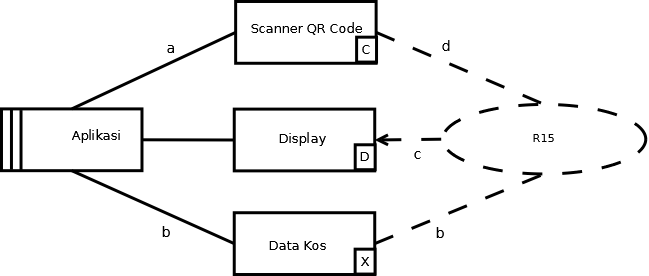
\includegraphics[scale=0.4]{gambar/7}
				\caption{\textit{Frame diagram: Information + Model Display}}
				\label{pb7}
			\end{figure}
		
	
		
			Berikut adalah penjelasan dari gambar \ref{pb7}.
			
			\begin{enumerate}[a.]
				\item App ! menyiapkan-\textit{scanner}
				
				SQC ! \textit{scanner}-disiapkan
				
				\item DK ! mengambil-data-kos
				
				\item D ! tampilkan-data-kos
				\item SQC ! membaca-\textit{qrcode}
			\end{enumerate}
			
			Artinya adalah Aplikasi menyiapkan \textit{scanner QR Code} untuk membaca \textit{QR Code} yang memuat informasi kos dimana data tersebut didapat dari Data Kos kemudian ditampilkan di Display Kos.
		\end{enumerate}
	
	\subsection{\textit{Class Diagram} dan \textit{ Object Constraint Language} (OCL)}
	Setelah mengumpulkan \textit{problem frames}, langkah selanjutnya adalah membuat \textit{class diagram} yang kemudian diterjemahkan ke dalam OCL. OCL akan menggambarkan aturan-aturan yang berlaku pada \textit{class diagram}. \textit{Class diagram} dan OCL akan memudahkan penulis dalam tahap pengkodean sistem. Gambar \ref{cdiagram} adalah \textit{class diagram} yang akan diterapkan pada sistem. \textit{Class diagram} terdiri dari nama kelas, atribut dan operasi. Sedangkan OCL terdiri dari konteks (context), invarian yaitu kondisi yang harus (hampir) selalu terpenuhi pada kelas, \textit{pre-condition} yaitu kondisi yang harus bernilai benar sebelum operasi dieksekusi dan \textit{post-condition} yaitu kondisi yang harus bernilai benar setelah operasi dieksekusi.

	\begin{figure}[H]
		\centering
		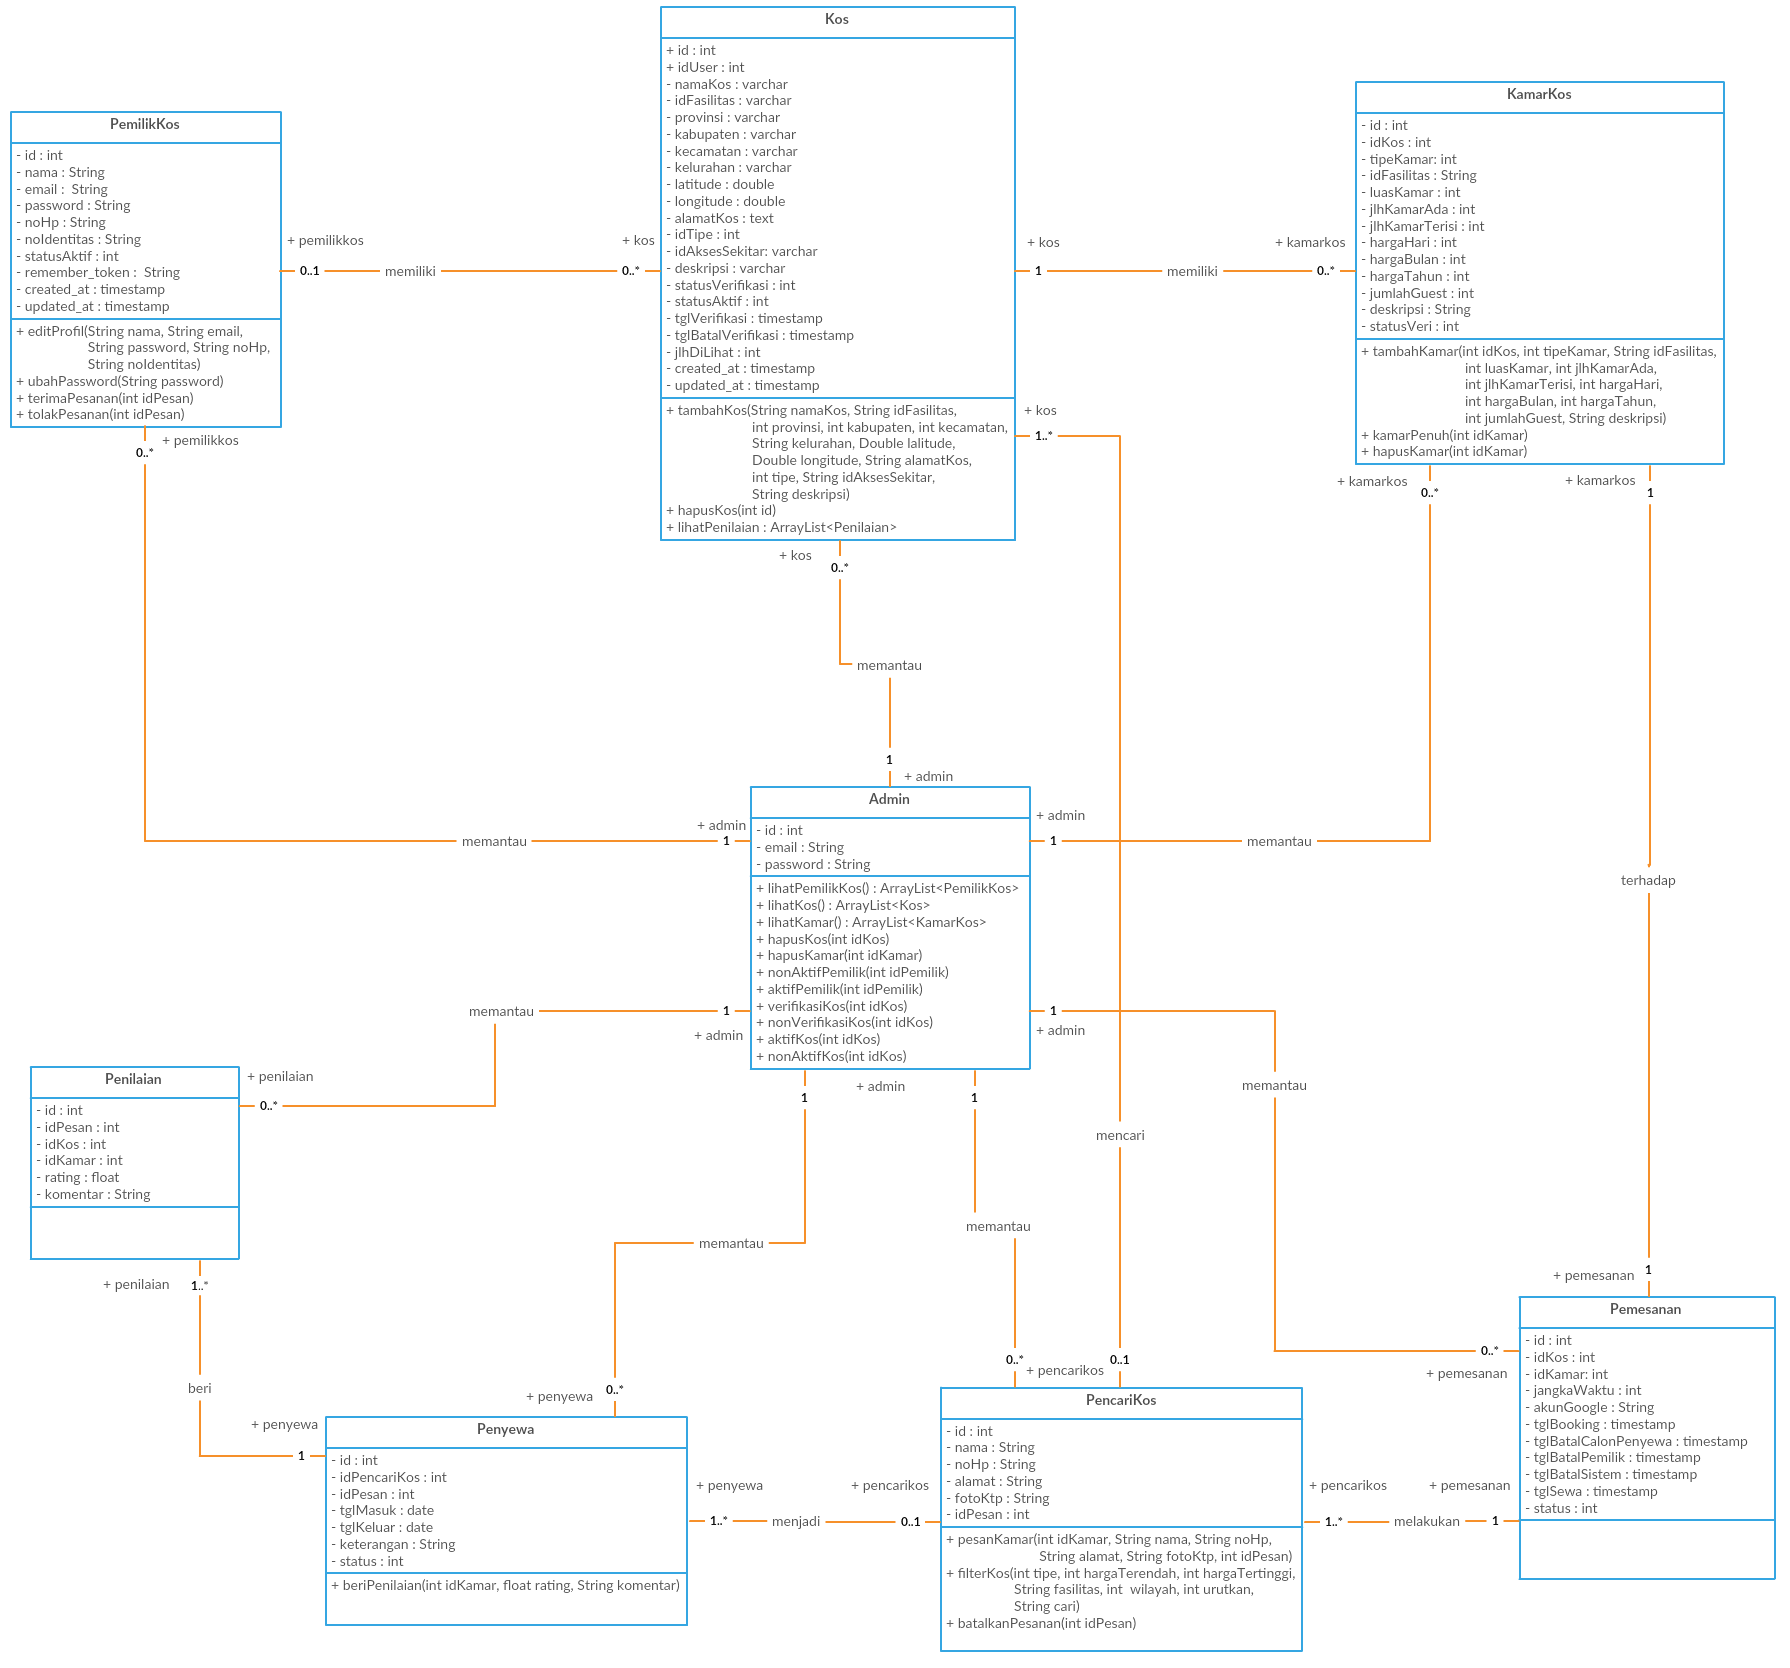
\includegraphics[scale=0.3]{gambar/classD}
		\caption{\textit{Class diagram yang diterapkan pada sistem}}
		\label{cdiagram}
	\end{figure}

	Berikut adalah aturan-aturan yang berlaku pada \textit{class diagram} yang diterjemahkan menggunakan OCL.
	
	\begin{figure}[H]
		\centering
		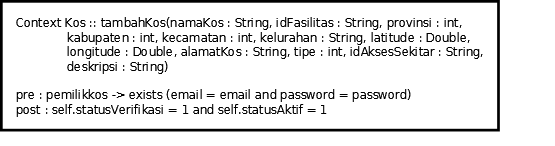
\includegraphics[scale=0.7]{gambar/ocl/tambahKos}
		\caption{OCL pada operasi penambahan data kos}
		\label{ocl1}
	\end{figure}

	Gambar \ref{ocl1} menjelaskan bahwa pada kelas Kos sebelum mengeksekusi operasi tambahKos, pemilik kos harus login terlebih dahulu, setelah tambahKos dieksekusi maka statusVerifikasi dan statusAktif pada kos tersebut bernilai 1. Artinya kos tersebut belum diverifikasi dan tidak akan ditampilkan pada aplikasi berbasis Android. Jadi setiap kos yang didaftarkan, tidak langsung tampil di aplikasi Android, tetapi harus melewati tahap verifikasi terlebih dahulu. Verifikasi dilakukan oleh admin dengan mengunjungi tempat kos, jika data yang dimasukkan benar, maka admin dapat memverifikasi kos tersebut dan muncul di aplikasi Android.
	
	\begin{figure}[H]
		\centering
		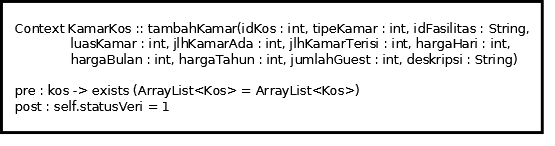
\includegraphics[scale=0.7]{gambar/ocl/tambahKamar}
		\caption{OCL pada operasi penambahan data kamar kos}
		\label{ocl2}
	\end{figure}

	Gambar \ref{ocl2} menjelaskan bahwa pada kelas KamarKos sebelum mengeksekusi operasi tambahKamar, data kos dari pemilik kos harus ada terlebih dahulu. Setelah operasi tambahKamar dieksekusi, statusVeri bernilai 1. Artinya pemilik kos harus memasukkan data kos terlebih dahulu sebelum menambahkan data kamar dan ketika menambahkan data kamar, statusVeri bernilai 1 yaitu kamar kos tidak tampil pada aplikasi Android. 
	
	\begin{figure}[H]
		\centering
		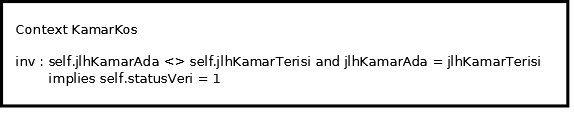
\includegraphics[scale=0.5]{gambar/ocl/KamarKos}
		\caption{OCL pada kelas KamarKos}
		\label{ocl3}
	\end{figure}

	Gambar \ref{ocl3} menjelaskan bahwa pada kelas KamarKos, jika atribut jlhKamarAda sama dengan jlhKamarTerisi maka statusVeri bernilai 1. Artinya jika kamar kos penuh, maka kamar tidak tampil pada aplikasi Android.
	
	\begin{figure}[H]
		\centering
		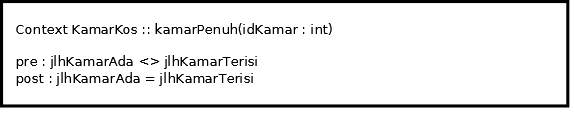
\includegraphics[scale=0.5]{gambar/ocl/kamarPenuh}
		\caption{OCL pada kelas KamarKos operasi kamarPenuh}
		\label{ocl4}
	\end{figure}
	
	Gambar \ref{ocl4} menjelaskan bahwa pada kelas KamarKos sebelum operasi kamarPenuh dieksekusi, jlhKamarAda tidak sama dengan jlhKamarTerisi dan setelah operasi kamarPenuh dieksekusi jlhKamarAda menjadi sama dengan jlhKamarTerisi dan statusVeri bernilai 1. Artinya tidak ada kamar yang akan disewa dan kamar tidak tampil pada aplikasi Android. 
	
	\begin{figure}[H]
		\centering
		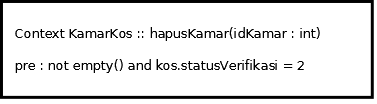
\includegraphics[scale=0.7]{gambar/ocl/hapuskamar}
		\caption{OCL pada kelas KamarKos operasi hapusKamar}
		\label{ocl5}
	\end{figure}
	
	Gambar \ref{ocl5} menjelaskan bahwa pada kelas KamarKos sebelum operasi hapusKamar dieksekusi, maka data kamar tidak boleh kosong dan statusVerifikasi pada kos harus bernilai 2. Artinya, menghapus kamar hanya bisa dilakukan jika data kamarnya ada dan kos belum diverifikasi oleh admin. Jika data kamar ada tetapi kos belum diverifikasi, maka tidak dapat menghapus kamar.
	
	\begin{figure}[H]
		\centering
		\includegraphics[scale=0.8]{gambar/ocl/hapusKos}
		\caption{OCL pada kelas Kos operasi hapusKos}
		\label{ocl6}
	\end{figure} 
	
	Gambar \ref{ocl6} menjelaskan bahwa pada kelas Kos sebelum operasi hapusKos dieksekusi, maka data kos tidak boleh kosong dan statusVerifikasi harus bernilai 2. Artinya sama seperti hapusKamar, menghapus kos hanya bisa dilakukan jika data kosnya ada dan kos belum diverifikasi oleh admin. Jika data kos ada tetapi kos belum diverifikasi, maka tidak dapat menghapus kos.
	
	\begin{figure}[H]
		\centering
		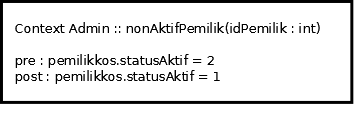
\includegraphics[scale=0.7]{gambar/ocl/nonAktifPemilik}
		\caption{OCL pada kelas Admin operasi nonAktifPemilik}
		\label{ocl7}
	\end{figure} 
	
	Gambar \ref{ocl7} menjelaskan bahwa pada kelas Admin sebelum operasi nonAktifPemilik dieksekusi, statusAktif dari pemilik kos harus bernilai 2. Dan setelah operasi nonAktifPemilik dieksekusi, statusAktif berubah menjadi 1. Artinya akun dari pemilik kos dapat dinonaktifkan jika sebelum dinonaktifkan, akun pemilik kos aktif dan setelah dinonaktifkan maka akun user menjadi tidak aktif. Akun pemilik kos yang tidak aktif menyebabkan pemilik kos tidak dapat login dan tidak dapat menggunakan aplikasi web.
	
	\begin{figure}[H]
		\centering
		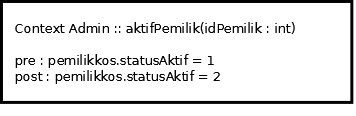
\includegraphics[scale=0.7]{gambar/ocl/aktifPemilik}
		\caption{OCL pada kelas Admin operasi aktifPemilik}
		\label{ocl8}
	\end{figure} 
	
	Gambar \ref{ocl8} menjelaskan bahwa pada kelas Admin sebelum operasi aktifPemilik dieksekusi, statisAktif dari pemilik kos harus bernilai 1. Dan setelah operasi aktifPemilik dieksekusi, statusAktif berubah menjadi 2. Artinya akun dari pemilik kos dapat diaktifkan jika sebelumnya akun tersebut nonaktif dan setelah diaktifkan maka akun pemilik kos menjadi aktif kembali.
	
	\begin{figure}[H]
		\centering
		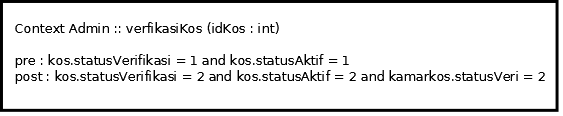
\includegraphics[scale=0.5]{gambar/ocl/verifikasikos}
		\caption{OCL pada kelas Admin operasi verifikasiKos}
		\label{ocl9}
	\end{figure} 
	
	Gambar \ref{ocl9} menjelaskan bahwa pada kelas Admin sebelum operasi verifikasiKos dieksekusi, statusVerifikasi dan statusAktif pada kos harus bernilai 1 dan setelah operasi verifikasiKos dieksekusi, maka statusVerifikasi dan statusAktif pada kos akan menjadi 2 serta statusVeri pada kamarKos akan menjadi 2 juga. Artinya untuk memverifikasi kos, maka sebelumnya kos belum diverifikasi dan tidak aktif. Setelah diverifikasi, maka kos menjadi terverifikasi dan muncul di aplikasi Android.
	
	\begin{figure}[H]
		\centering
		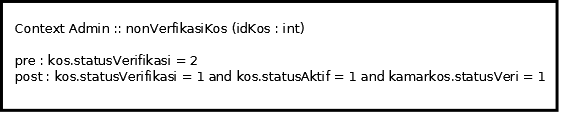
\includegraphics[scale=0.5]{gambar/ocl/nonVerifikasikos}
		\caption{OCL pada kelas Admin operasi nonVerifikasiKos}
		\label{ocl10}
	\end{figure} 
	
	Gambar \ref{ocl10} menjelaskan bahwa pada kelas Admin sebelum operasi nonVerifikasiKos dieksekusi, statusVerifikasi pada kos harus bernilai 2 dan setelah operasi verifikasiKos dieksekusi, maka statusVerifikasi dan statusAktif pada kos akan menjadi 1 serta statusVeri pada kamarKos akan menjadi 1 juga. Artinya untuk membatalkan verifikasi kos, maka sebelumnya kos sudah diverifikasi. Setelah dibatalkan verifikasi, maka kos menjadi tidak terverifikasi dan tidak muncul di aplikasi Android.
	
	\begin{figure}[H]
		\centering
		\includegraphics[scale=0.5]{gambar/ocl/aktifKos}
		\caption{OCL pada kelas Admin operasi aktifKos}
		\label{ocl11}
	\end{figure} 
	
	Gambar \ref{ocl11} menjelaskan bahwa pada kelas Admin sebelum operasi aktifKos dieksekusi, statusVerifikasi pada kos harus bernilai 2 dan statusAktif pada kos bernilai 1. Setelah operasi aktifKos dieksekusi, maka statusVerifikasi dan statusAktif pada kos akan menjadi 2 serta statusVeri pada kamarKos akan menjadi 2 juga. Artinya mengaktifkan kos hanya bisa dilakukan untuk kos yang sudah diverifikasi tetapi tidak aktif (tidak muncul pada aplikasi Android). Sehingga setelah diaktifkan, kos akan muncul di aplikasi Android.
	
	\begin{figure}[H]
		\centering
		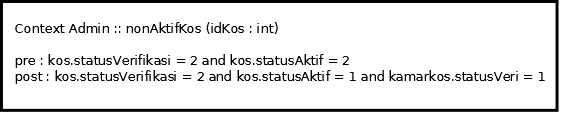
\includegraphics[scale=0.5]{gambar/ocl/nonAktifKos}
		\caption{OCL pada kelas Admin operasi nonAktifKos}
		\label{ocl12}
	\end{figure} 
	
	Gambar \ref{ocl12} menjelaskan bahwa pada kelas Admin sebelum operasi nonAktifKos dieksekusi, statusVerifikasi dan statusAktif pada kos harus bernilai 2. Setelah operasi nonAktifKos dieksekusi, maka statusVerifikasi pada kos akan menjadi 2, statusAktif pada kos menjadi 1 dan statusVeri pada kamarKos menjadi 1. Artinya menonaktifkan kos hanya bisa dilakukan untuk kos yang sudah diverifikasi dan aktif (muncul pada aplikasi Android). Sehingga setelah dinonaktifkan, kos tidak akan muncul di aplikasi Android.

	\begin{figure}[H]
		\centering
		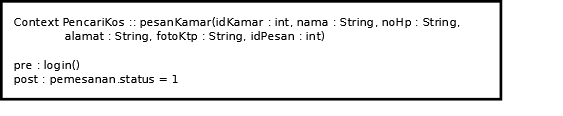
\includegraphics[scale=0.7]{gambar/ocl/pesankamar}
		\caption{OCL pada kelas PencariKos operasi pesanKamar}
		\label{ocl12a}
	\end{figure}

	Gambar \ref{ocl12a} menjelaskan bahwa pada kelas PencariKos sebelum operasi pesanKamar dieksekusi, pencari kos harus login terlebih dahulu. Setelah operasi pesanKamar dieksekusi, maka status pada pemesanan menjadi 1. Status bernilai 1 pada kelas Pemesanan adalah "baru dipesan". 

	\begin{figure}[H]
		\centering
		\includegraphics[scale=0.5]{gambar/ocl/batalKanPesanan}
		\caption{OCL pada kelas PencariKos operasi batalKanPesanan}
		\label{ocl13}
	\end{figure}
	
	Gambar \ref{ocl13} menjelaskan bahwa pada kelas PencariKos sebelum operasi batalkanPesanan dieksekusi, status pada pemesanan harus bernilai 1. Kemudian setelah operasi batalkanPesanan dieksekusi, maka status di pemesanan berubah menjadi 2. Artinya untuk membatalkan pemesanan, pencari kos harus memesan kamar terlebih dahulu. Status bernilai 2 pada kelas Pemesanan adalah "dibatalkan oleh pencari kos". 
	
	\begin{figure}[H]
		\centering
		\includegraphics[scale=0.5]{gambar/ocl/terimaPesanan}
		\caption{OCL pada kelas PemilikKos operasi terimaPesanan}
		\label{ocl14}
	\end{figure}
	
	Gambar \ref{ocl14} menjelaskan bahwa pada kelas PemilikKos sebelum operasi terimaPesanan dieksekusi, status pada pemesanan harus bernilai 1. Kemudian setelah operasi terimaPesanan dieksekusi, maka status di pemesanan berubah menjadi 5. Artinya kamar kos dari pemilik kos harus dipesan dahulu sebelum dapat diterima. Status bernilai 5 pada kelas Pemesanan adalah "diterima oleh pemilik kos".
	
	\begin{figure}[H]
		\centering
		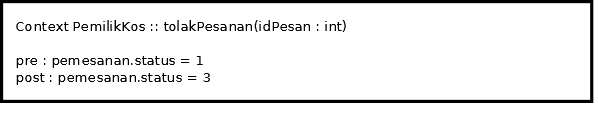
\includegraphics[scale=0.5]{gambar/ocl/tolakPesanan}
		\caption{OCL pada kelas PemilikKos operasi tolakPesanan}
		\label{ocl15}
	\end{figure}
	
	Gambar \ref{ocl15} menjelaskan bahwa pada kelas PemilikKos sebelum operasi tolakPesanan dieksekusi, status pada pemesanan harus bernilai 1. Kemudian setelah operasi tolakPesanan dieksekusi, maka status di pemesanan berubah menjadi 3. Artinya kamar kos dari pemilik kos harus dipesan dahulu sebelum dapat ditolak. Status bernilai 3 pada kelas Pemesanan adalah "dibatalkan oleh pemilik kos".
	
	\begin{figure}[H]
		\centering
		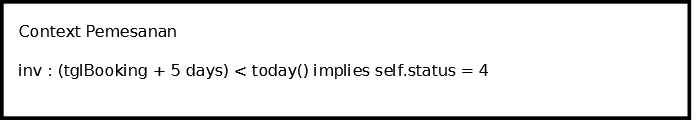
\includegraphics[width=\textwidth]{gambar/ocl/batalsistem}
		\caption{OCL pada kelas Pemesanan}
		\label{ocl16}
	\end{figure}
	
	Gambar \ref{ocl16} menjelaskan bahwa pada kelas Pemesanan setiap tanggal \textit{booking} jika lebih dari 5 hari, maka pemesanan akan dibatalkan oleh sistem.
	
	\begin{figure}[H]
		\centering
		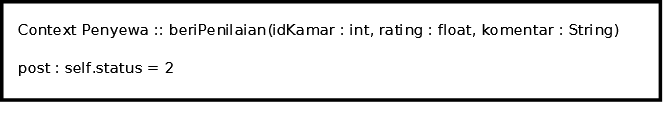
\includegraphics[width=\textwidth]{gambar/ocl/beripenilaian}
		\caption{OCL pada kelas Penyewa operasi beriPenilaian}
		\label{ocl17}
	\end{figure}
	
	Gambar \ref{ocl17} menjelaskan bahwa pada kelas Penyewa setelah operasi beriPenilaian dieksekusi, maka status penyewa menjadi 2. Artinya penyewa sudah memberikan penilaian terhadap kos, dan tidak dapat mengubah penilaian tersebut.
	
	\section{Perancangan Sistem}
		Perancangan sistem dimulai dengan membuat \textit{ERD Diagram}. \textit{ERD Diagram }akan menggambarkan relasi-relasi antara basis data. Gambar \ref{erd} adalah \textit{ERD Diagram }yang diterapkan pada aplikasi ini.
		
		\begin{landscape}
			\begin{figure}[H]
				\centering
				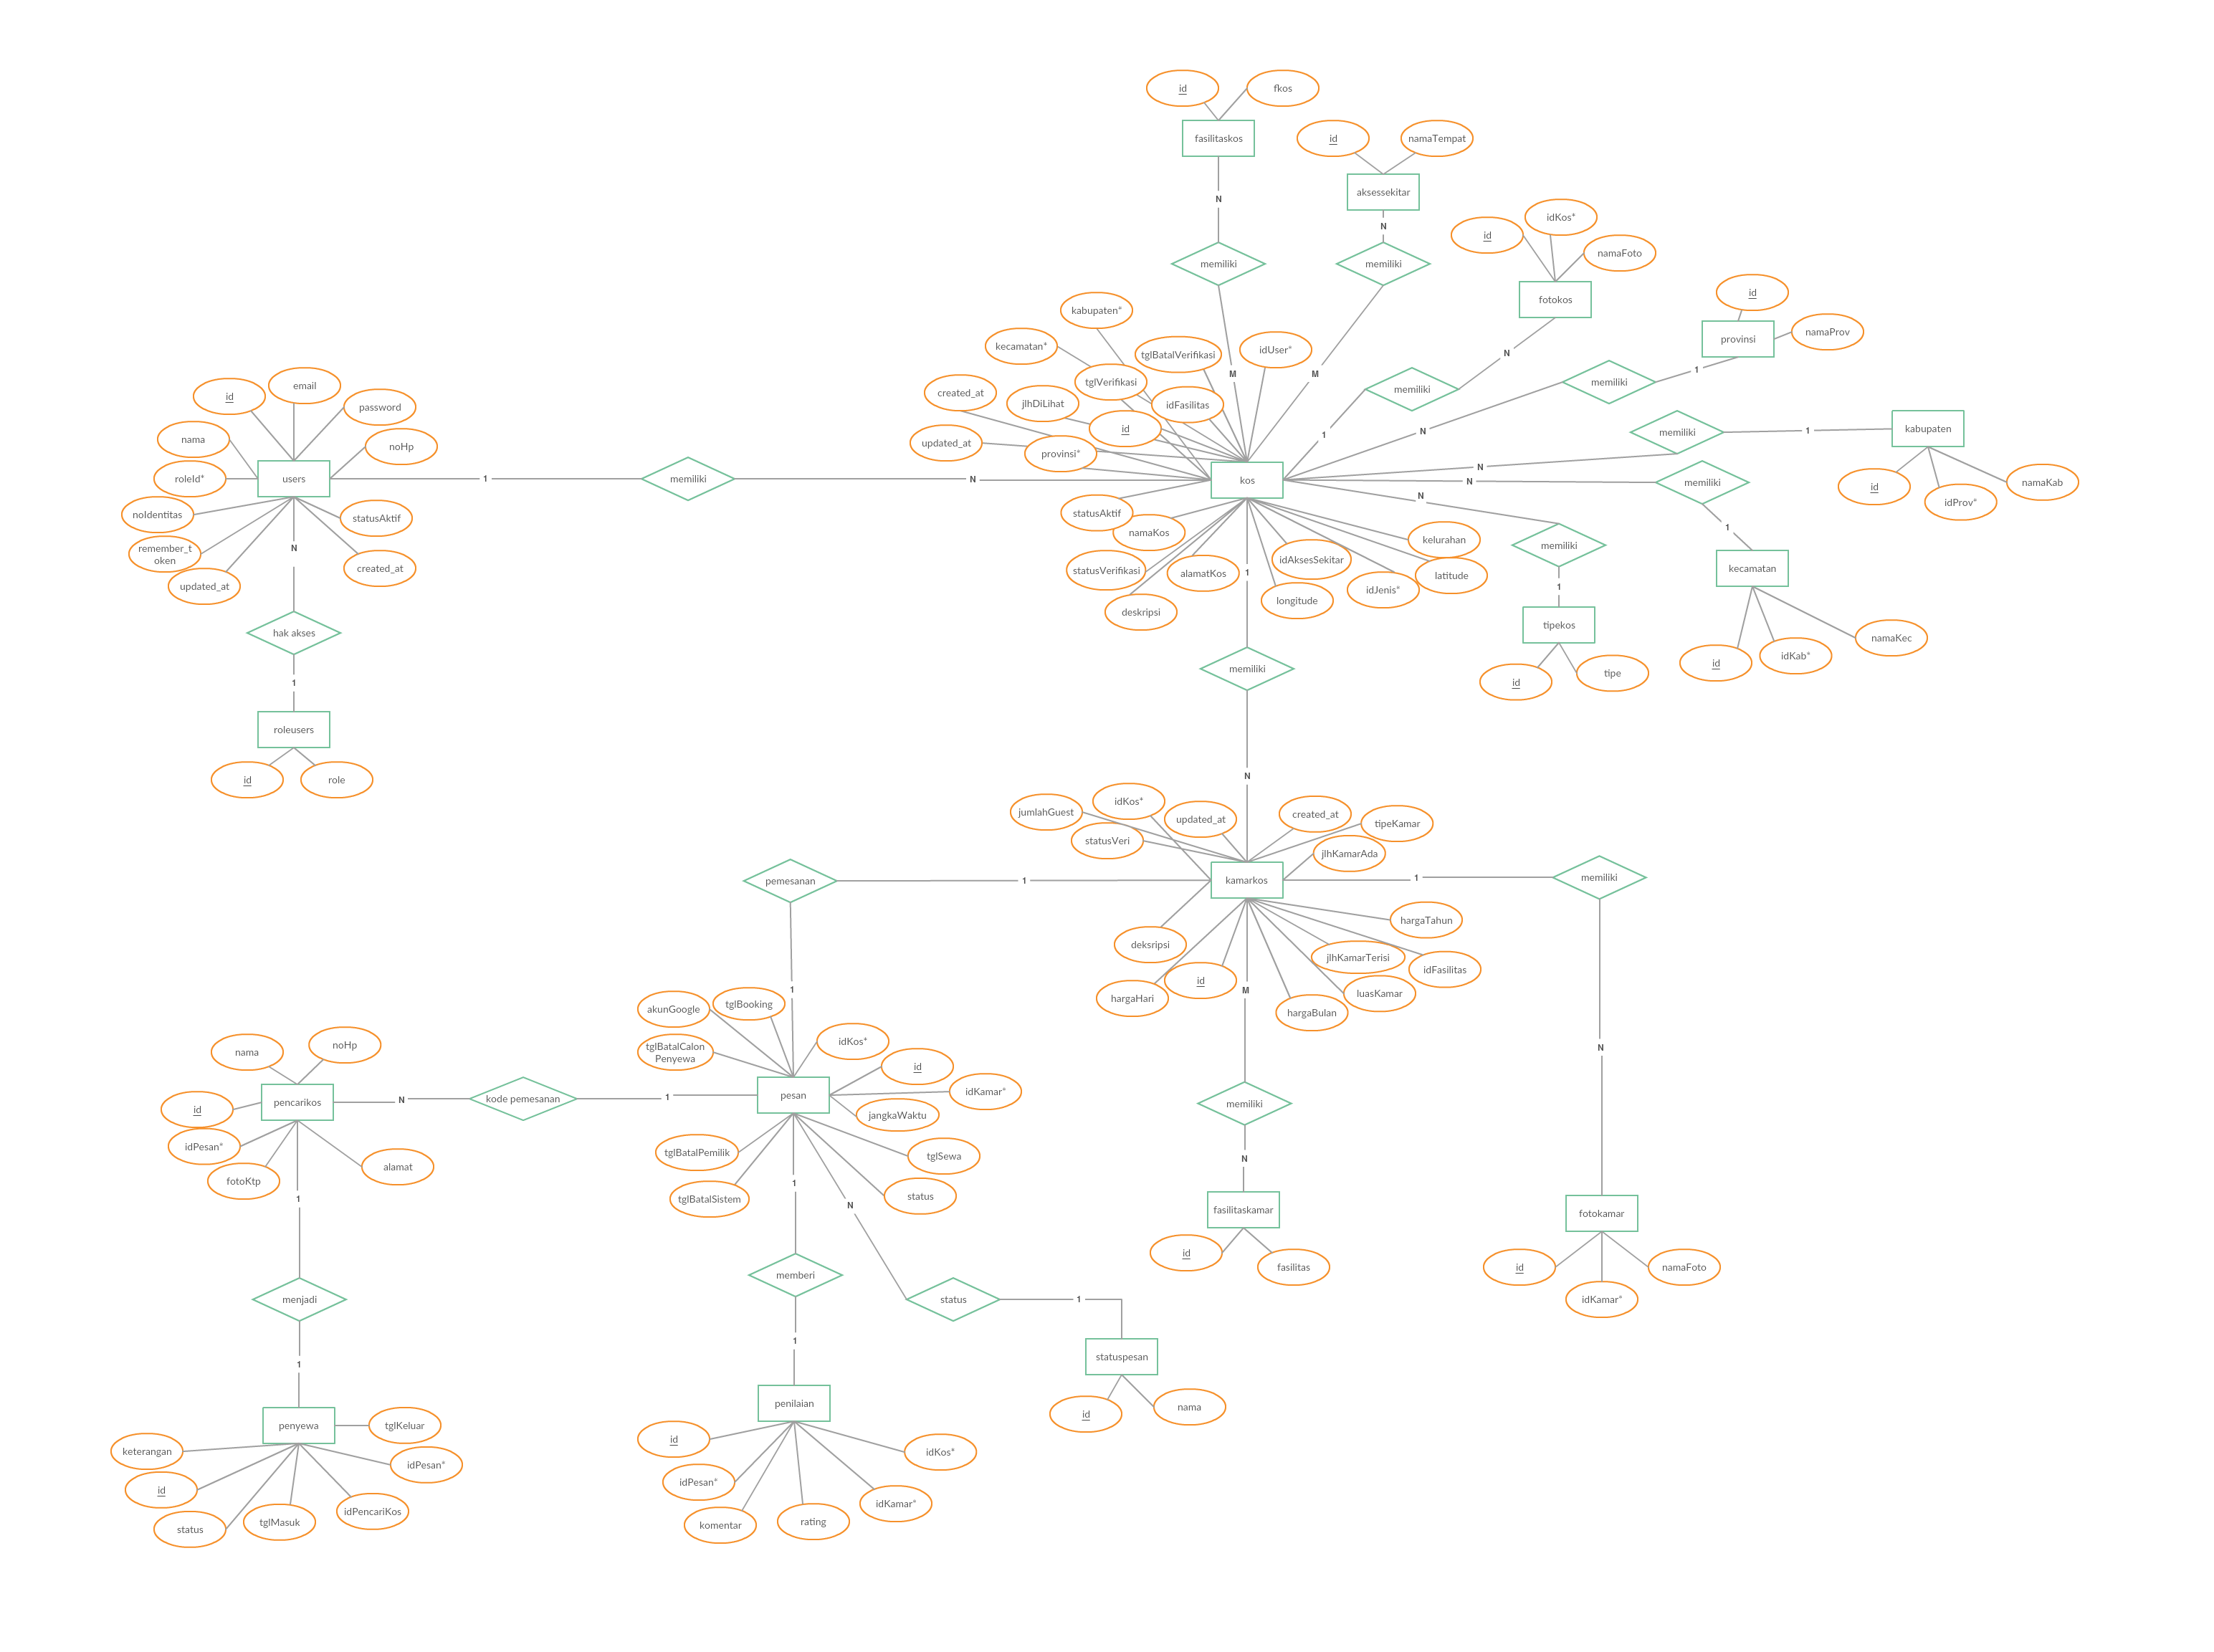
\includegraphics [width = 24cm, height= 13cm]{gambar/erd2}
				\caption{ERD yang diterapkan pada aplikasi}
				\label{erd}
			\end{figure}
		\end{landscape}
	
		Untuk memahami penggunaan aplikasi kos-kosan, berikut adalah gambaran atau proses yang terjadi dengan membuat \textit{flowchart}. 
		
		\begin{enumerate}[a.]
			\item Pemilik kos
			
			Pemilik kos dapat melakukan tambah data kos (bisa lebih dari satu) dan tambah data kamar (bisa lebih dari satu). Data kos dan data kamar yang sudah didaftarkan, belum muncul pada aplikasi Android karena akan ditinjau terlebih dahulu oleh admin dan admin akan melakukan survey langsung ke kos tersebut. Jika data yang dimasukkan benar, maka admin akan memverifikasi data kos dan langsung muncul di aplikasi Android. Pemilik kos juga dapat melihat berapa orang yang telah melihat kos miliknya dan orang-orang yang memesan kamar kos. Pemilik kos atau pencari kos dapat saling menghubungi untuk membahas kesepakatan penyewaan dan pembayaran uang sewa. Pemilik kos dapat menyetujui atau menolak penyewaan kamar kos miliknya dan dapat melihat daftar orang-orang yang menyewa kamar kos miliknya serta penilaian dari penyewa tersebut.
			
			Pemilik kos menggunakan aplikasi berbasis web. Gambar \ref{flow1} adalah proses menggunakan aplikasi kos-kosan yang ditujukan pada pemilik kos.
			\begin{landscape}
				\begin{figure}[H]
					\centering
					\includegraphics [width = 24cm, height= 13cm]{gambar/ocl/diagrampemilik}
					\caption{\textit{Flowchart} Pemilik Kos}
					\label{flow1}
				\end{figure}
			\end{landscape}
		
			\item Pencari kos
			
			Pencari kos dapat melihat daftar kos-kosan yang ada, dapat memilih kos berdasarkan jenis kos, rentang harga, fasilitas dan dapat mengurutkan harga dari harga terendah ke harga tertinggi dan sebaliknya. Pencari kos dapat melihat informasi detail tentang kos dan kamar kos yang diminatinya serta dapat melihat lokasi kos melalui peta. Pencari kos dapat memesan kamar kos dengan memasukkan data diri beserta foto KTP. Pemilik kos atau pencari kos dapat saling menghubungi untuk membahas kesepakatan penyewaan dan pembayaran uang sewa. Namun, jika terjadi salah pemesanan atau hal lainnya, pencari kos dapat membatalkan pemesanan. Jika pemesanan di terima oleh pemilik kos, maka pencari kos akan menjadi penyewa kos. 
			
			Pencari kos menggunakan aplikasi berbasis Android. Gambar \ref{flow2} adalah proses menggunakan aplikasi kos-kosan yang ditujukan pada pencari kos.
			 
			\begin{figure}[H]
				\centering
				\includegraphics[width=\textwidth]{gambar/ocl/diagramuser}
				\caption{\textit{Flowchart} Pencari Kos}
				\label{flow2}
			\end{figure}
		
		\item Admin
		
		Admin bertugas untuk memverifikasi kos agar dapat ditampilkan di aplikasi Android. Sebelum verifikasi dilakukan, admin akan melihat data kos yang terdaftar, kemudian melakukan survey langsung ke kos tersebut. Jika data kos tersebut benar, maka admin akan memverifikasi kos. Jika data kos tidak benar, maka admin dapat memberi tahu pemilik kos untuk mengubah datanya atau admin tidak akan memverifikasi kos tersebut. Verfikasi kos dilakukan untuk mengurangi kepalsuan data yang dapat merugikan pencari kos. Jika kos sudah diverifikasi, maka kos tersebut dapat tampil di aplikasi Android. Selain memverifikasi kos, admin dapat menon-aktifkan akun pemilik kos, menon-aktifkan kos dan dapat menghapus kos dan kamar kos. Hal ini dapat dilakukan jika terjadi kecurangan, merugikan orang lain atau bahkan permintaan pemilik kos sendiri.
		
		Admin menggunakan aplikasi berbasis web.  Gambar \ref{flow3} adalah proses aplikasi web untuk admin.
		
		\begin{landscape}
			\begin{figure}[H]
				\centering
				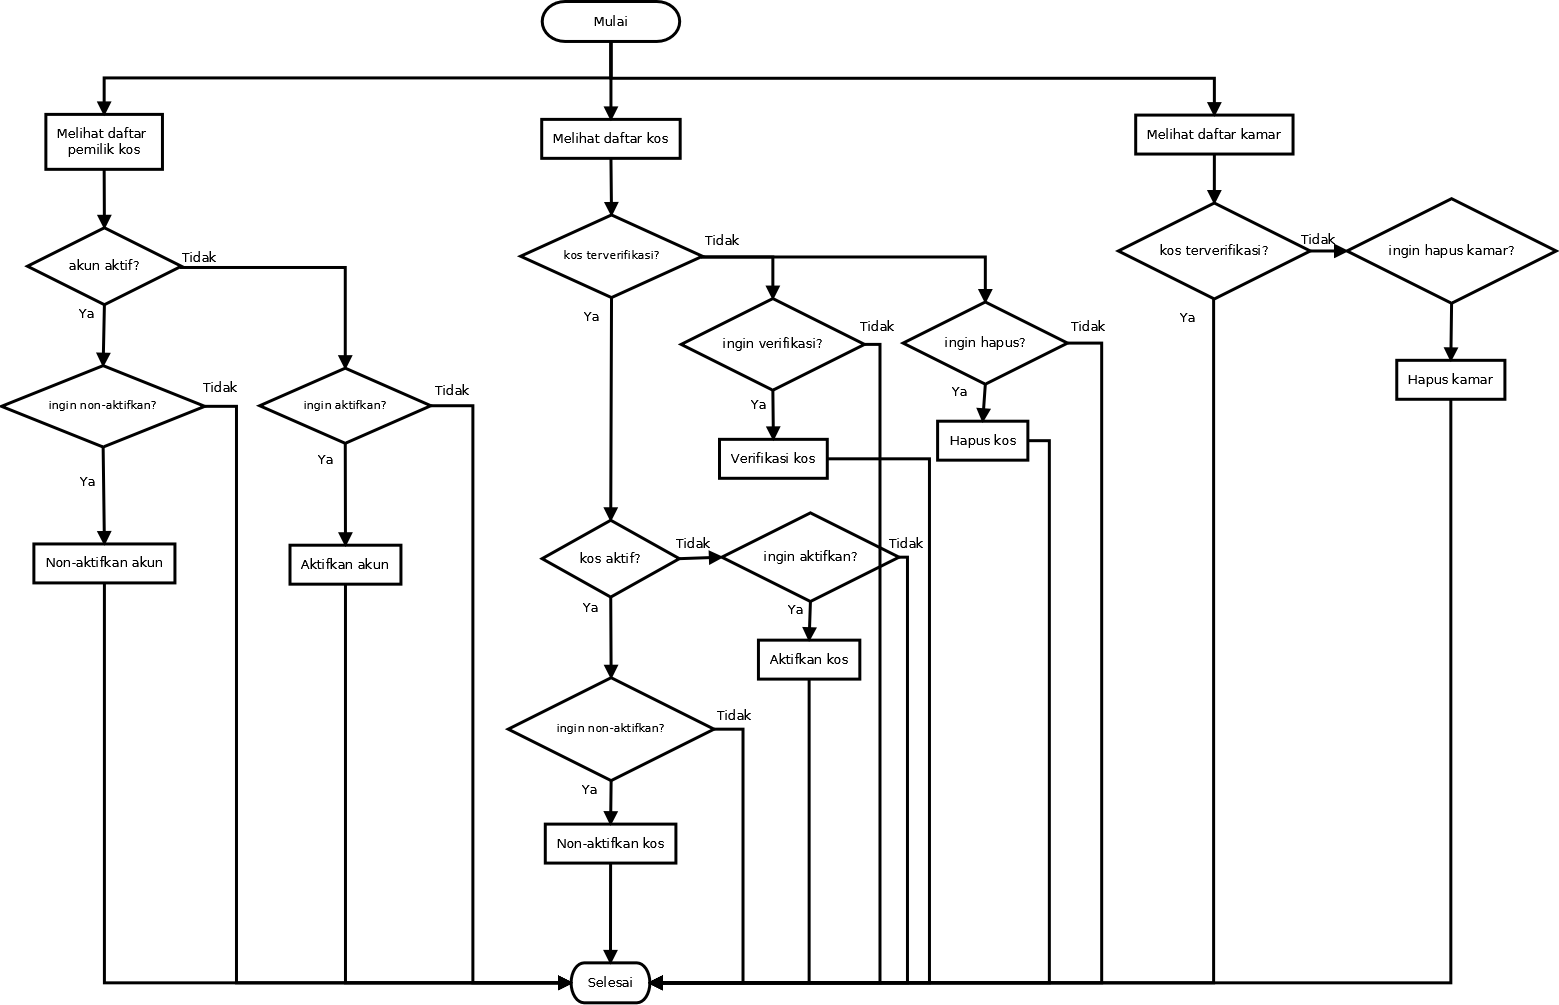
\includegraphics [width = 24cm, height= 13cm]{gambar/ocl/flowAdmin}
				\caption{\textit{Flowchart} admin}
				\label{flow3}
			\end{figure}
		\end{landscape}
		
		\end{enumerate}
	
	\section{Pengkodean Sistem}
	Aplikasi yang dibangun berbasis web dan Android. Aplikasi web digunakan oleh admin dan pemilik kos serta aplikasi Android digunakan oleh pencari kos. Pembuatan aplikasi web menggunakan bahasa PHP dengan \textit{framework} Laravel dan basis data yang digunakan adalah MySql. Sedangkan untuk Android menggunakan bahasa pemrograman Java. 
	
	\subsection{Tampilan Aplikasi Web}

		\begin{enumerate}[a.]
			\item Pemilik Kos
		
		\begin{figure}[H]
			\centering
			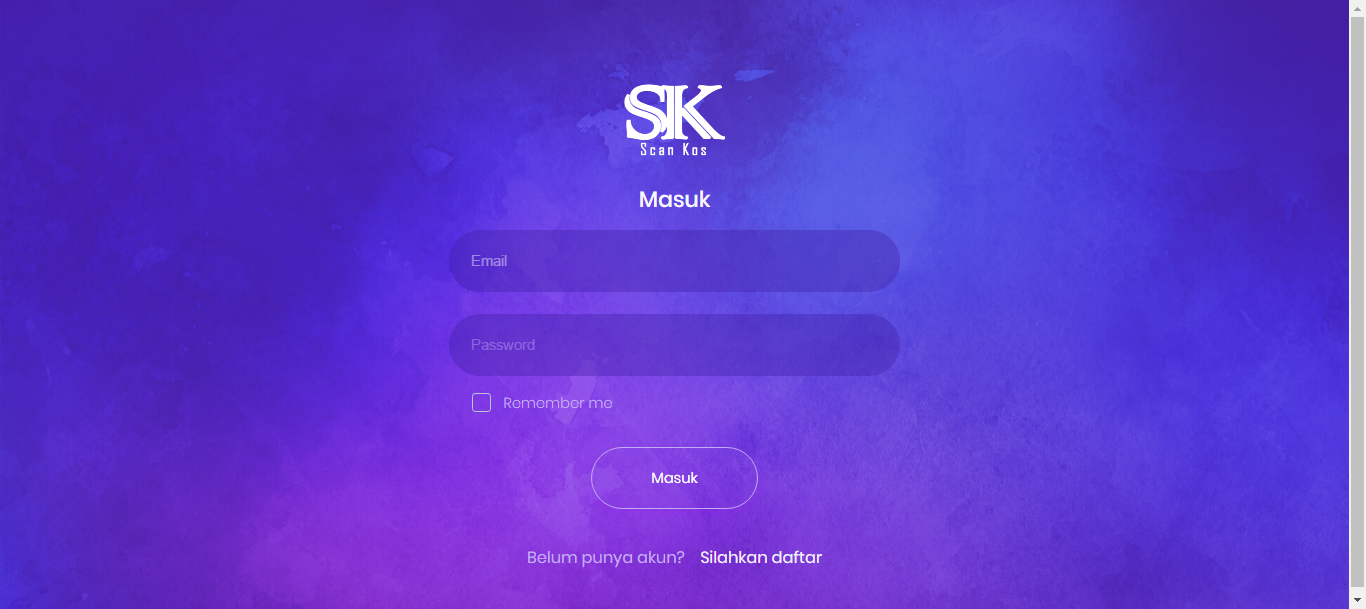
\includegraphics[width=\textwidth]{gambar/web/1}
			\caption{Halaman \textit{login}}
			\label{web1}
		\end{figure}
	
		Gambar \ref{web1} adalah halaman \textit{login}. Jika pemilik kos belum memiliki akun, maka pemilik kos harus mendaftarkan dirinya terlebih dahulu.
	
		\begin{figure}[H]
			\centering
			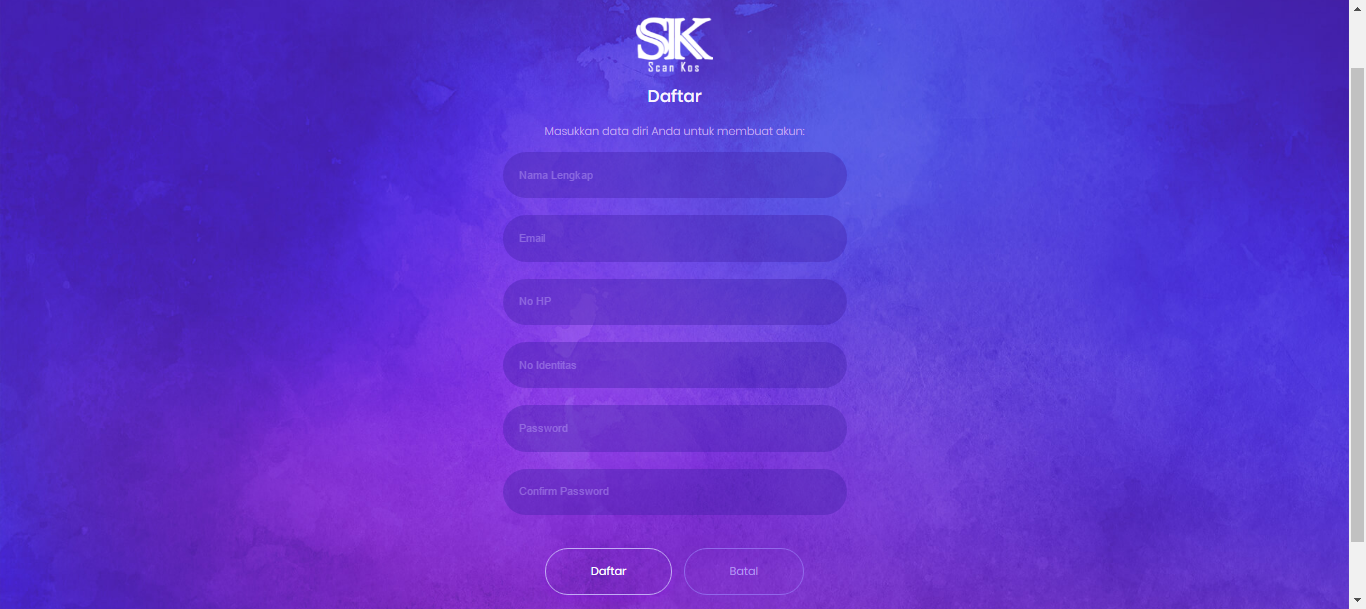
\includegraphics[width=\textwidth]{gambar/web/2}
			\caption{Halaman \textit{login}}
			\label{web2}
		\end{figure}
		
		Gambar \ref{web2} adalah halaman daftar. Setelah mendaftarkan akun, maka pemilik kos dapat melakukan \textit{login}.
		
		\begin{figure}[H]
			\centering
			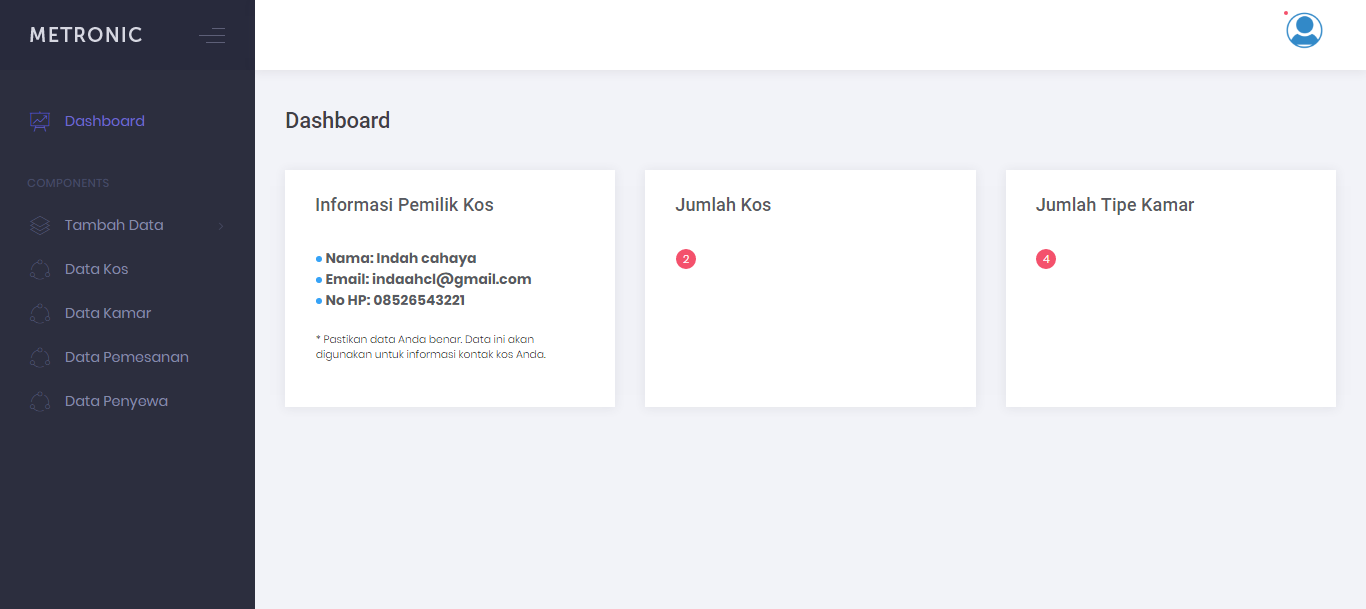
\includegraphics[width=\textwidth]{gambar/web/3}
			\caption{Halaman awal}
			\label{web3}
		\end{figure}
		
		Gambar \ref{web3} adalah halaman awal ketika pemilik kos \textit{login}. Pada halaman ini akan memuat informasi pemilik kos yang akan ditampilkan pada aplikasi Android, jumlah kos serta jumlah tipe kamar. 
		
		\begin{figure}[H]
			\centering
			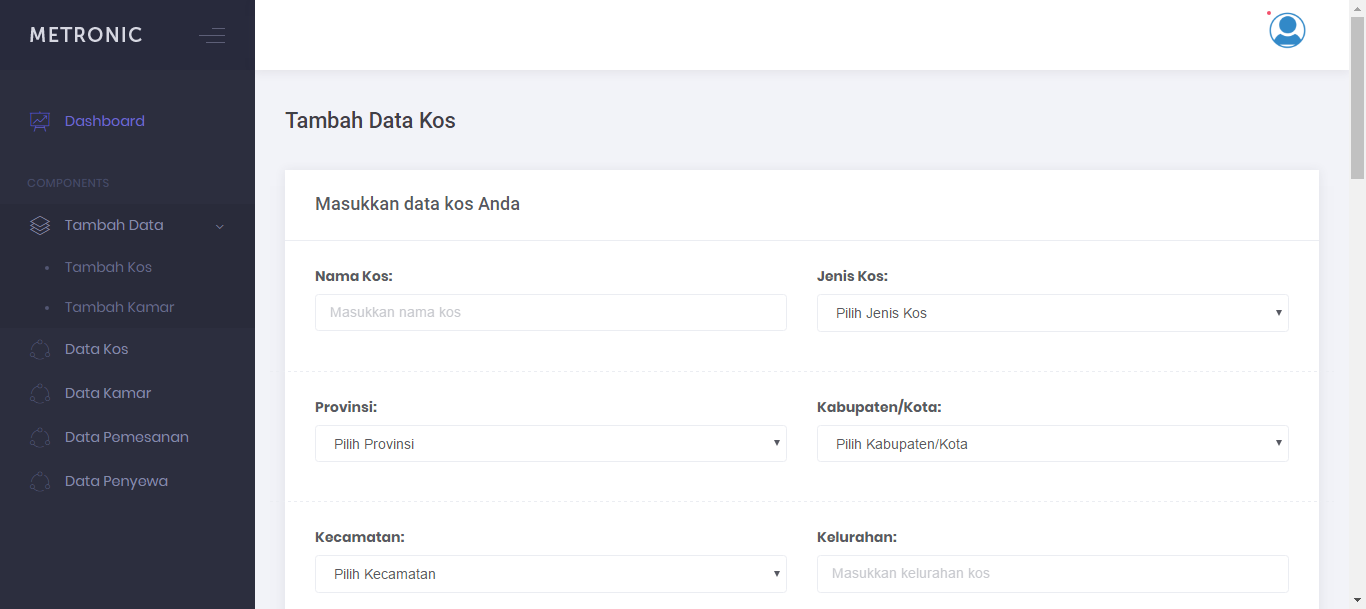
\includegraphics[width=\textwidth]{gambar/web/4}
			\caption{Halaman menambahkan data kos}
			\label{web4}
		\end{figure}
	
		\begin{figure}[H]
			\centering
			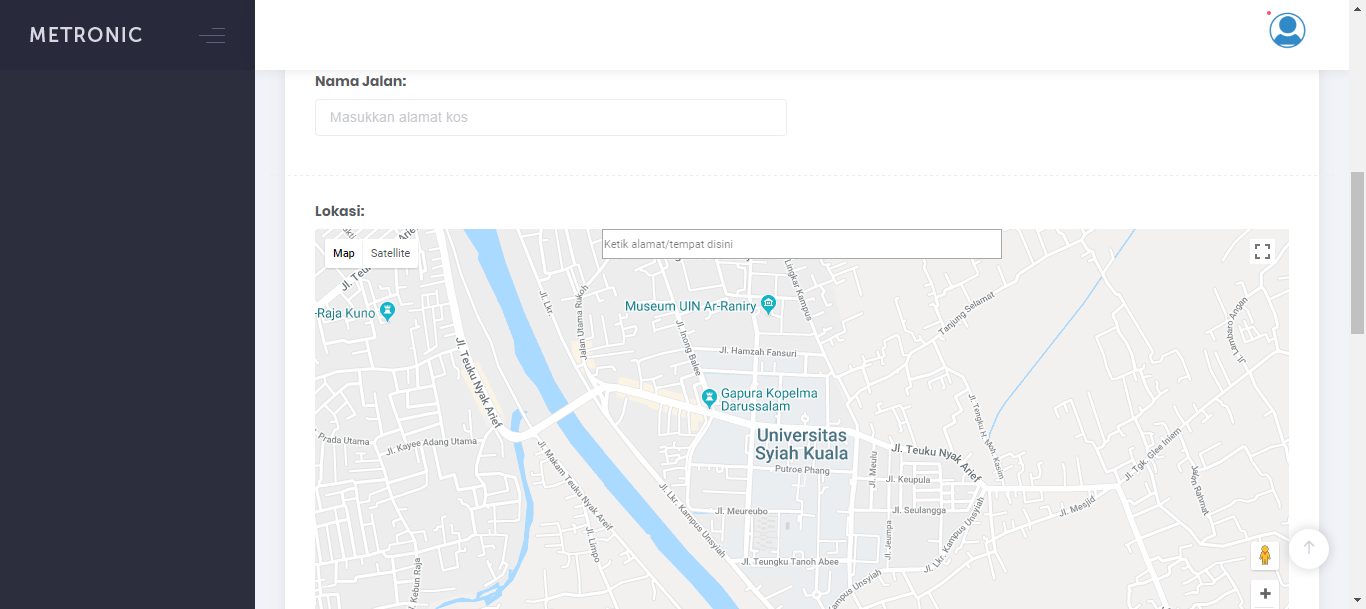
\includegraphics[width=\textwidth]{gambar/web/5}
			\caption{Halaman menambahkan data kos}
			\label{web5}
		\end{figure}
	
		\begin{figure}[H]
			\centering
			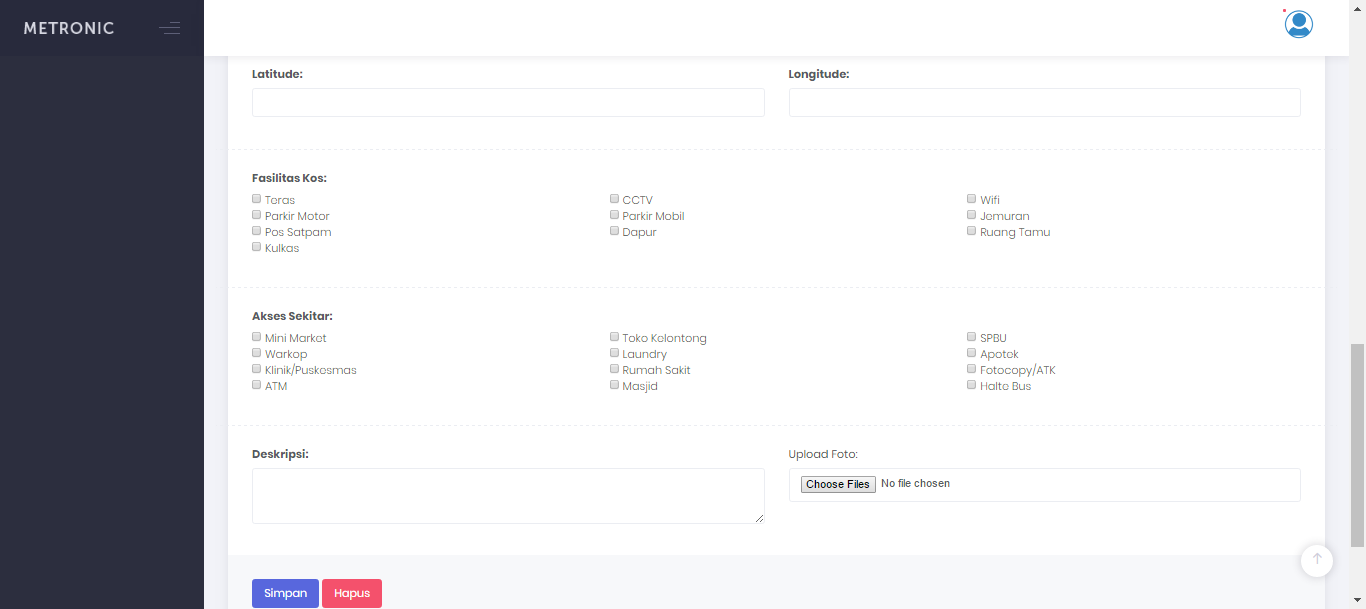
\includegraphics[width=\textwidth]{gambar/web/6}
			\caption{Halaman menambahkan data kos}
			\label{web6}
		\end{figure}
			
		Gambar \ref{web4}, \ref{web5} dan \ref{web6} adalah halaman untuk menambahkan data kos. Terdapat beberapa hal yang harus diisi oleh pemilik kos seperti nama kos, jenis kos, alamat lengkap kos, koordinat peta, fasilitas kos, akses sekitar, deksripsi dan foto. Setelah menambahkan kos, selanjutnya adalah menambahkan data kamar dari kos yang di-\textit{input} sebelumnya. Pemilik kos dapat menambahkan lebih dari satu kos.
		
		\begin{figure}[H]
			\centering
			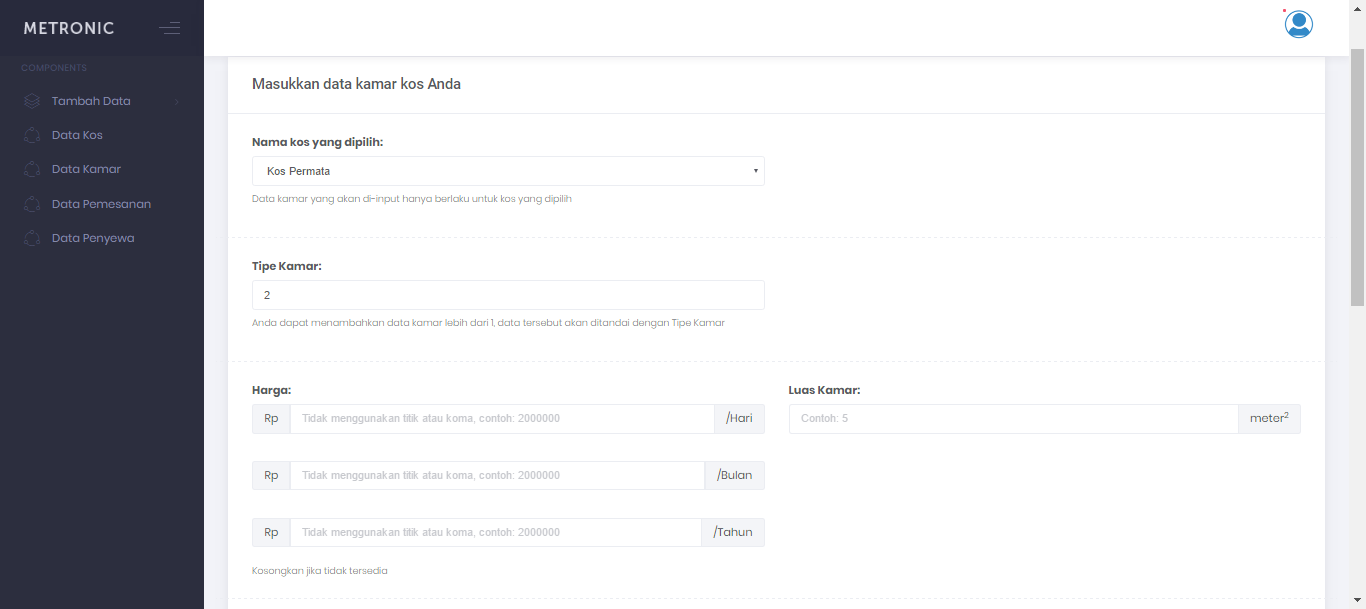
\includegraphics[width=\textwidth]{gambar/web/7}
			\caption{Halaman menambahkan data kamar kos}
			\label{web7}
		\end{figure}
	
		\begin{figure}[H]
			\centering
			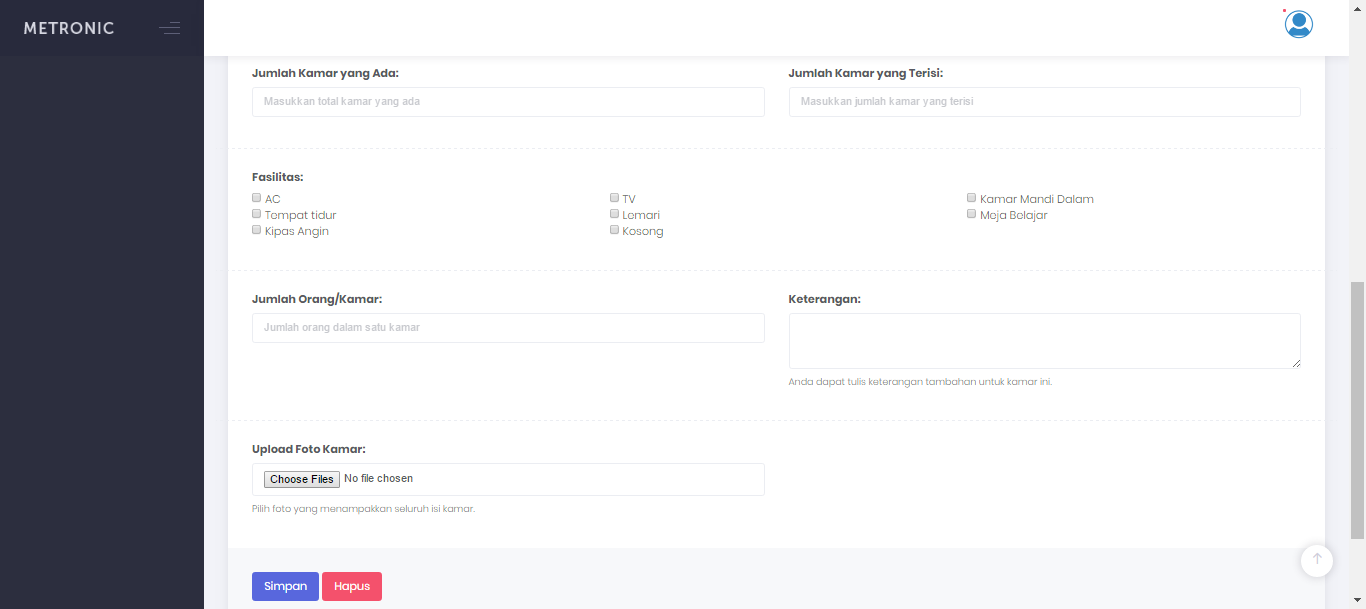
\includegraphics[width=\textwidth]{gambar/web/8}
			\caption{Halaman menambahkan data kamar kos}
			\label{web8}
		\end{figure}
		
		Gambar \ref{web7} adalah halaman untuk menambahkan data kamar kos. Jika pemilik kos memiliki banyak kos, pemilik kos dapat memilih kos mana yang akan dimasukkan data kamarnya. Dan setelah memilih kos, maka otomatis akan keluar tipe berapa kamar tersebut. Terdapat beberapa hal yang harus dimasukkan datanya oleh pemilik kos, seperti harga hari, bulan dan tahun (jika tidak ada, dapat dikosongkan),  luas kamar kos, jumlah kamar yang ada pada kos, jumlah kamar yang telah disewa, fasilitas kamar, jumlah orang perkamar, keterangan lainnya yang berkaitan dengan kamar dan terakhir adalah foto kamar.
	
		\begin{figure}[H]
			\centering
			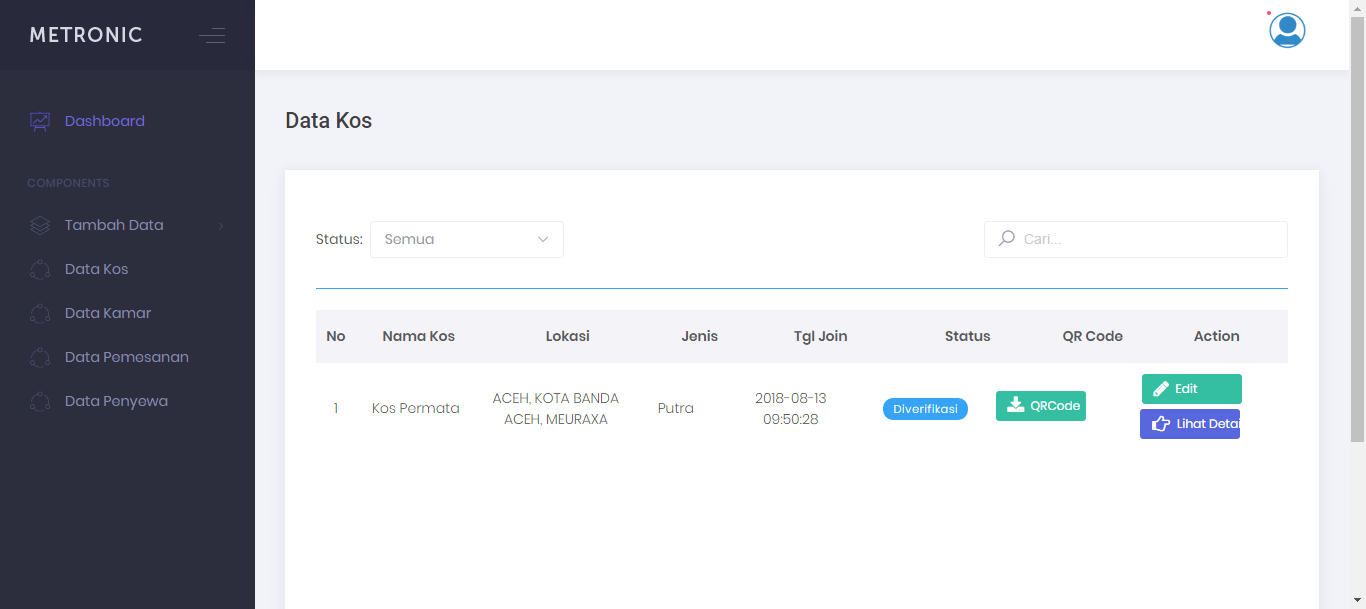
\includegraphics[width=\textwidth]{gambar/web/9}
			\caption{Halaman data semua kos}
			\label{web9}
		\end{figure}
		
		Gambar \ref{web9} adalah halaman yang memuat semua kos yang dimasukkan oleh pemilik kos. Terdapat menu QR Code, Edit serta Lihat Detail pada halaman ini.
		
	
		\begin{figure}[H]
			\centering
			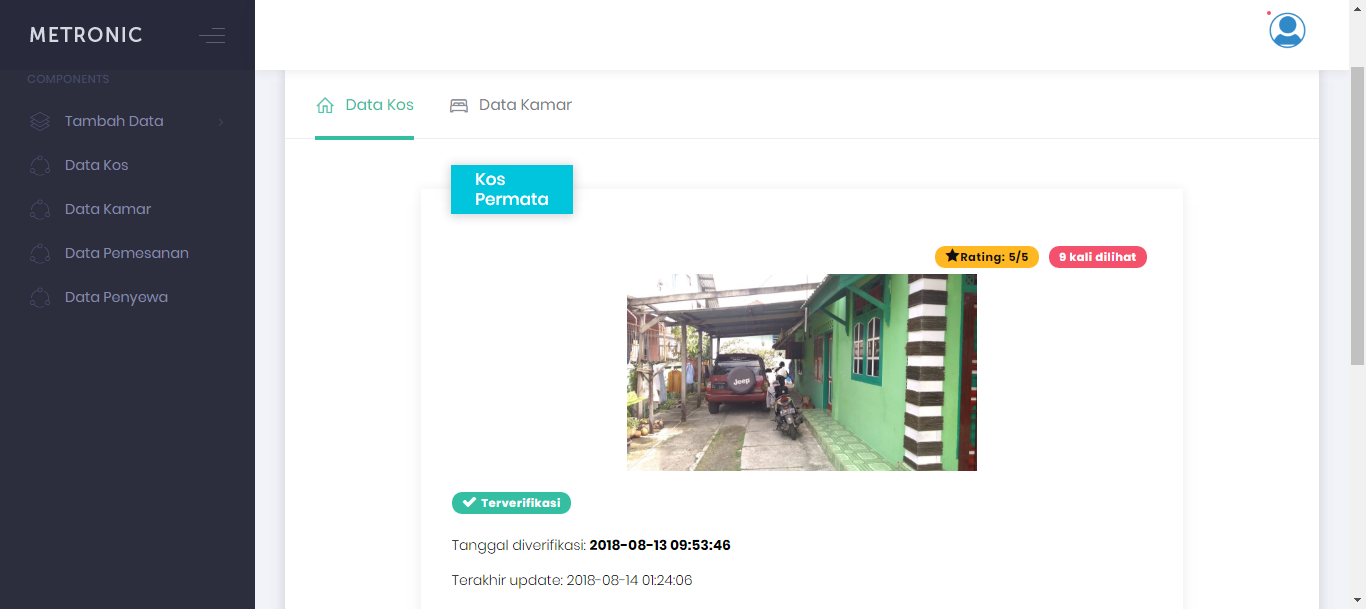
\includegraphics[width=\textwidth]{gambar/web/17}
			\caption{Halaman detail data kos}
			\label{web17}
		\end{figure}
	
		\begin{figure}[H]
			\centering
			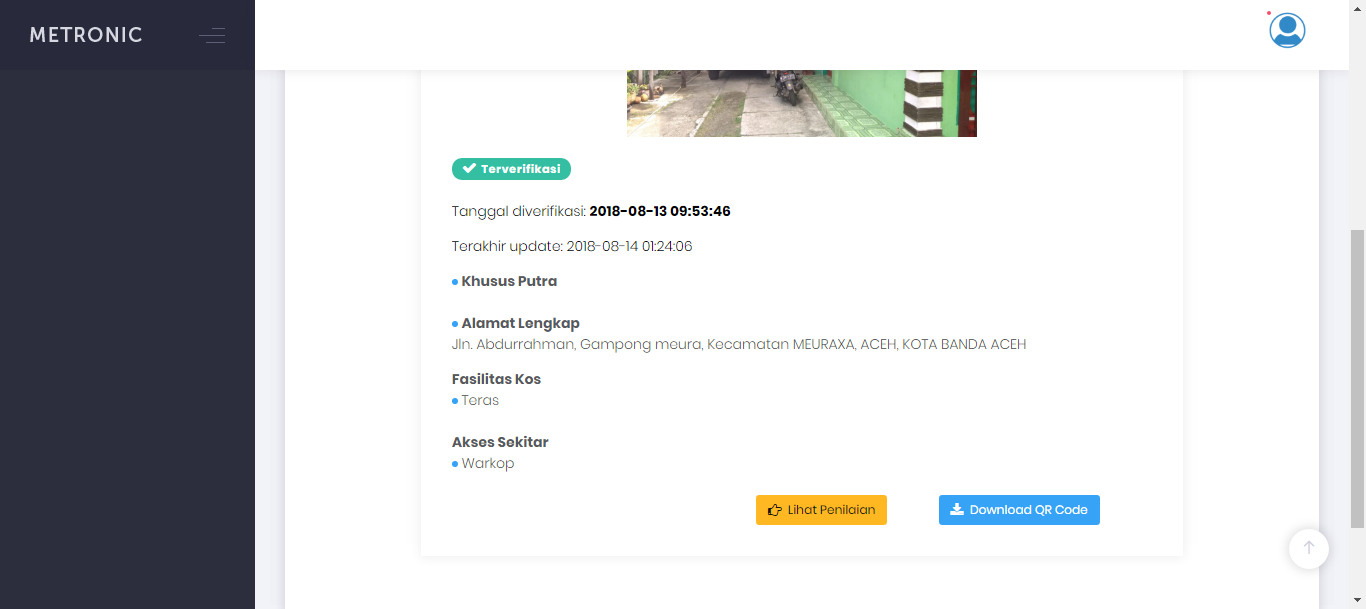
\includegraphics[width=\textwidth]{gambar/web/18}
			\caption{Halaman detail data kos}
			\label{web18}
		\end{figure}
		
		Gambar \ref{web17} dan \ref{web18} adalah halaman yang menampilkan detail dari kos yang di-\textit{input}. Pemilik kos dapat melihat status dari kosnya, apakah sudah diverifikasi oleh admin atau belum. Selain itu, pemilik kos dapat mengetahui jumlah orang yang melihat kos miliknya. Jika kos sudah diverifikasi, maka pemilik kos dapat melihat dan mengunduh \textit{QR Code} yang didalamnya terdapat informasi mengenai kos miliknya. \textit{QR Code} dapat dimanfaatkan oleh pemilik kos untuk ditempel di dinding terluar kos, sehingga pencari kos dapat memindai \textit{QR Code} tersebut dengan menggunakan aplikasi Android. Selain itu, jika kos sudah pernah dipesan dan sudah diberi penilaian, pemilik kos dapat melihat penilaian tersebut.
		
		\begin{figure}[H]
			\centering
			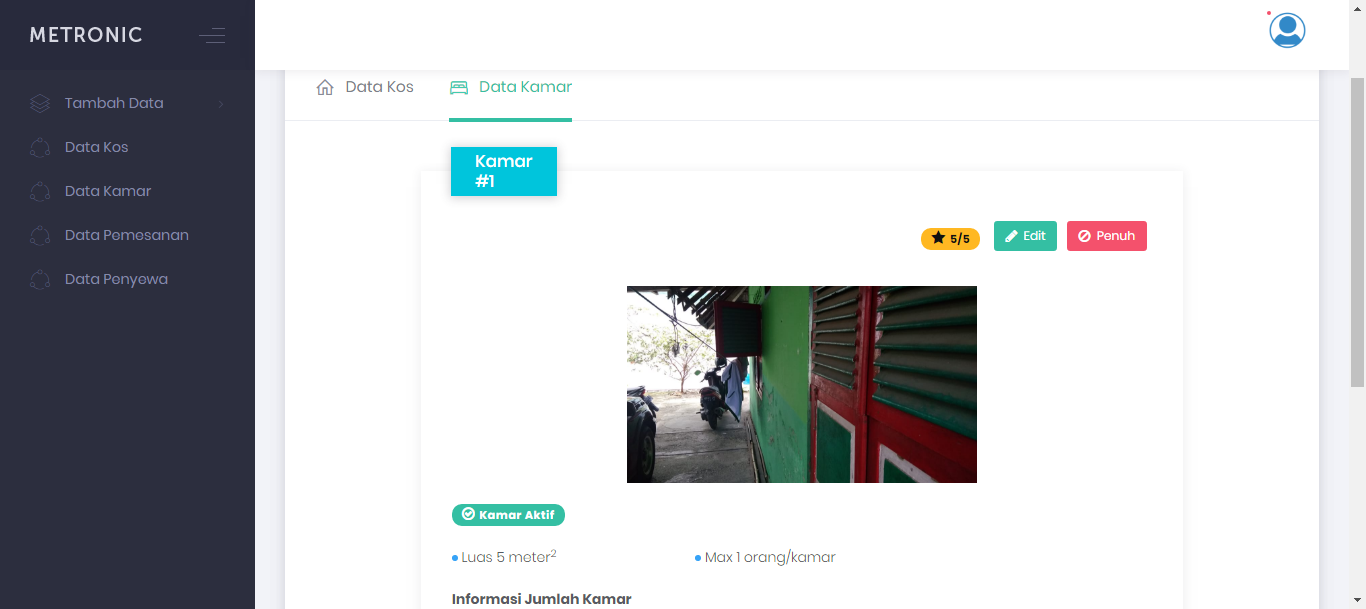
\includegraphics[width=\textwidth]{gambar/web/19}
			\caption{Halaman detail data kamar kos}
			\label{web19}
		\end{figure}
	
		Gambar \ref{web19} adalah halaman yang menampilkan detail dari kamar kos yang di-\textit{input}. Pemilik kos dapat melihat bintang kamar yang diberikan oleh penyewa. Terdapat tombol Edit dan Penuh pada halaman ini, edit digunakan untuk mengubah data yang diperlukan sedangkan tombol penuh digunakan jika kamar kos sudah tidak ada kamar untuk disewa.
		
		\begin{figure}[H]
			\centering
			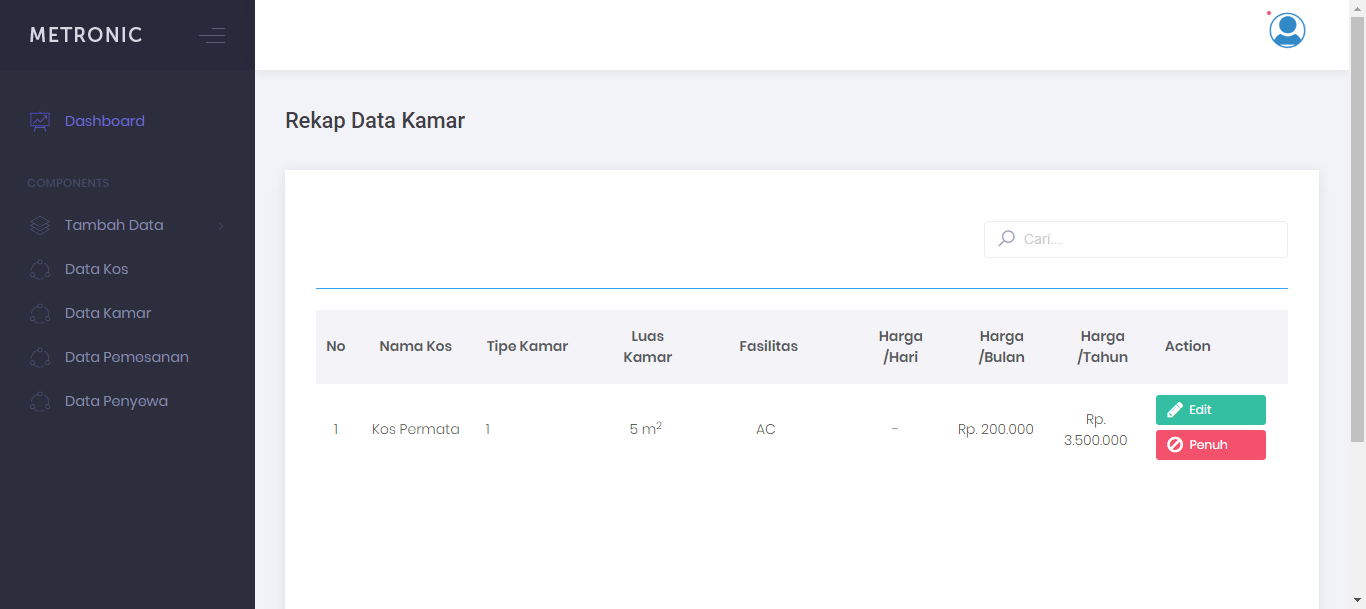
\includegraphics[width=\textwidth]{gambar/web/10}
			\caption{Halaman data kamar kos}
			\label{web10}
		\end{figure}
	
		Gambar \ref{web10} adalah halaman yang memuat semua kamar kos.
		
		\begin{figure}[H]
			\centering
			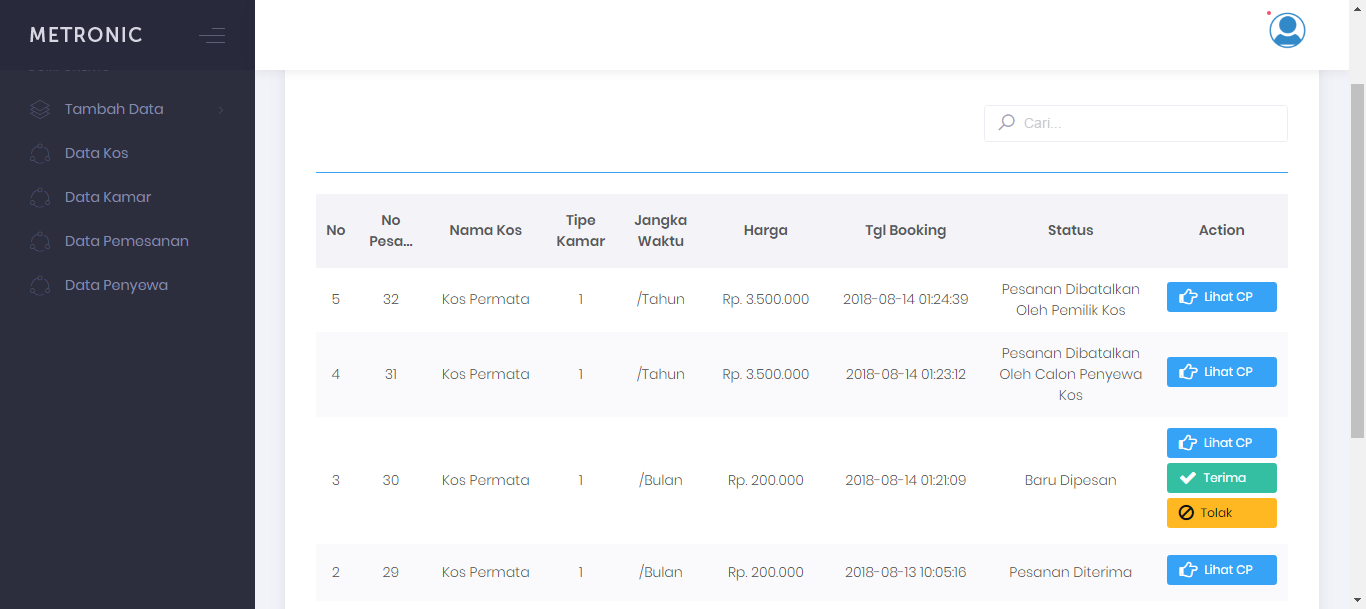
\includegraphics[width=\textwidth]{gambar/web/12}
			\caption{Halaman pemesanan kamar kos}
			\label{web12}
		\end{figure}
	
		Gambar \ref{web12} adalah halaman yang memuat semua daftar pemesanan kamar kos. Pada halaman ini pemilik kos dapat mengetahui status dari pemesanan. Terdapat 5 status pada pemesanan, yaitu:
		
		\begin{enumerate}[-]
			\item Baru dipesan
			\item Pesanan dibatalkan oleh calon penyewa kos
			\item Pesanan dibatalkan oleh pemilik kos
			\item Pesanan dibatalkan oleh sistem
			\item Pesanan diterima
		\end{enumerate}
	
		Pemilik kos dapat menerima dan menolak calon penyewa kos. Namun sebelumnya, diharapkan pemilik kos dapat menghubungi calon penyewa kos untuk melakukan kontak secara langsung atau calon penyewa kos juga dapat menghubungi pemilik kos. Kontak langsung yang dimaksud adalah calon penyewa kos dapat mendatangi kos dan mendiskusikan mengenai penyewaan kos. Jika calon penyewa dan pemilik kos saling setuju dan melakukan transaksi, maka langkah selanjutnya adalah pemilik kos menerima calon penyewa pada aplikasi. Namun jika tidak terjadi kesepakatan antara kedua belah pihak, maka pemilik kos dapat menolak calon penyewa atau bahkan calon penyewa dapat membatalkan pesanan melalui aplikasi Android.
		
		\begin{figure}[H]
			\centering
			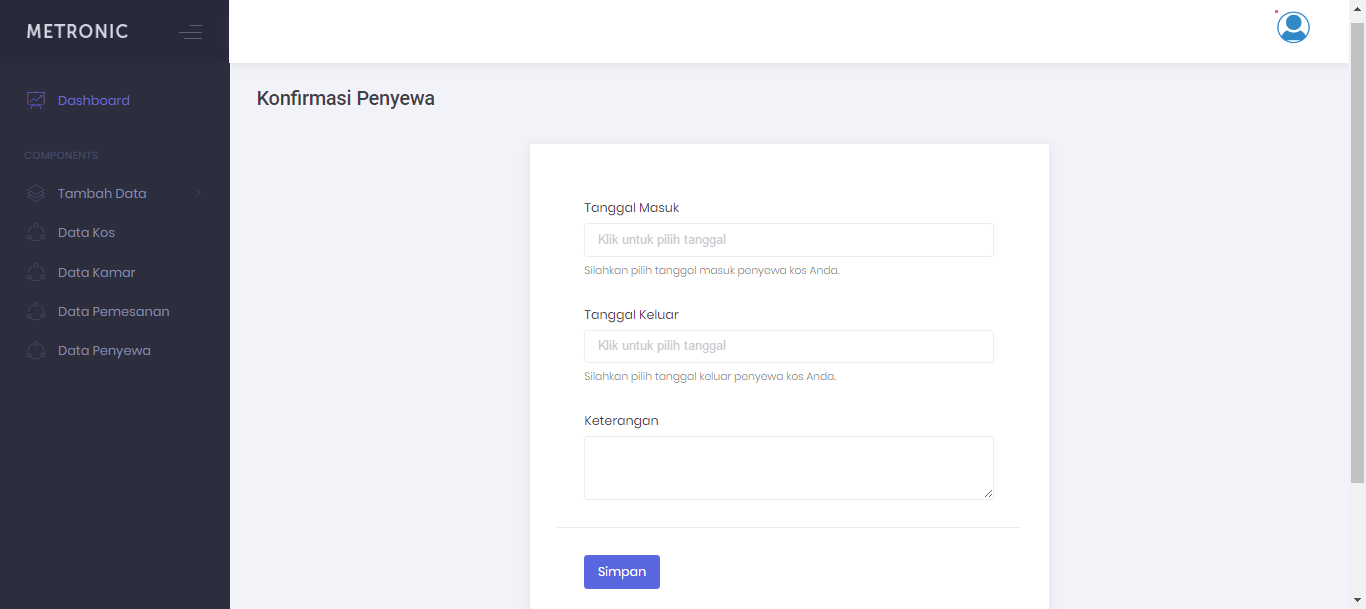
\includegraphics[width=\textwidth]{gambar/web/13}
			\caption{Halaman terima calon penyewa}
			\label{web13}
		\end{figure}
		
		Gambar \ref{web13} adalah halaman ketika pemilik kos menerima calon penyewa dan dapat mengisi tanggal masuk dan keluar serta keterangan tambahan lainnya.
		
		\begin{figure}[H]
			\centering
			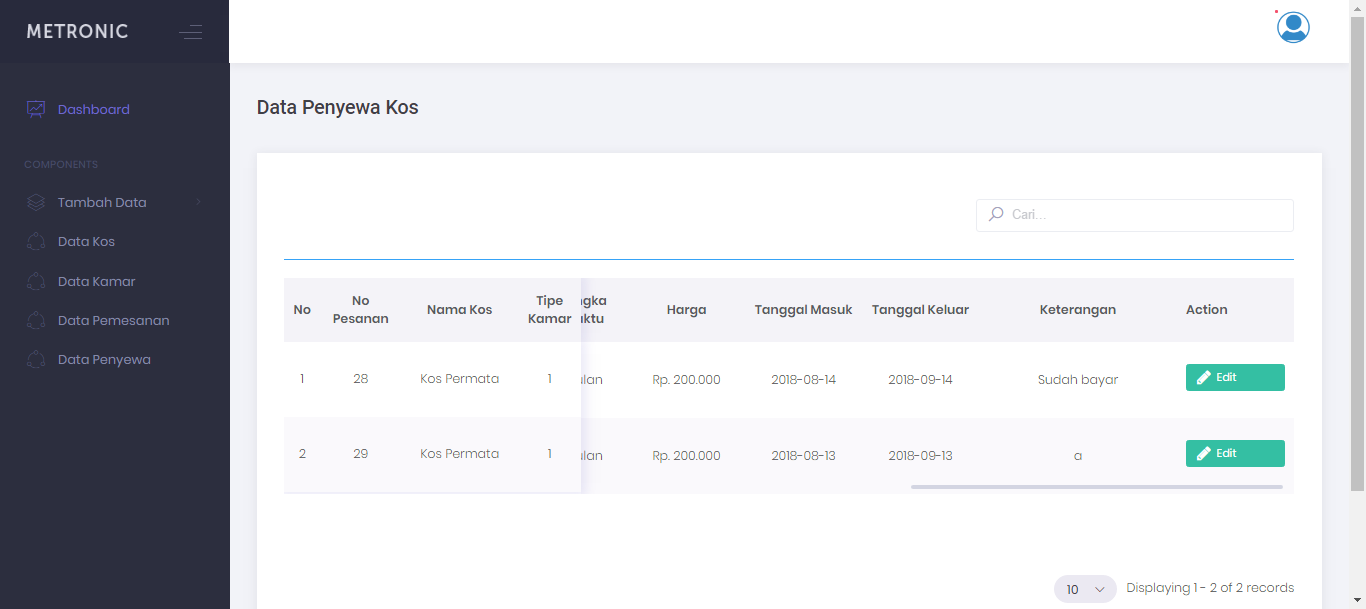
\includegraphics[width=\textwidth]{gambar/web/14}
			\caption{Halaman daftar penyewa}
			\label{web14}
		\end{figure}
		
		Gambar \ref{web14} adalah halaman yang memuat semua penyewa yang telah melakukan pemesanan melalui aplikasi Android. Pada halaman ini, pemilik kos dapat mengedit penyewa, yaitu tanggal keluar dan keterangan jika ada penyewa yang tiba-tiba tidak menyewa sebelum masa sewa habis.
		
		\item Admin
		\begin{figure}[H]
			\centering
			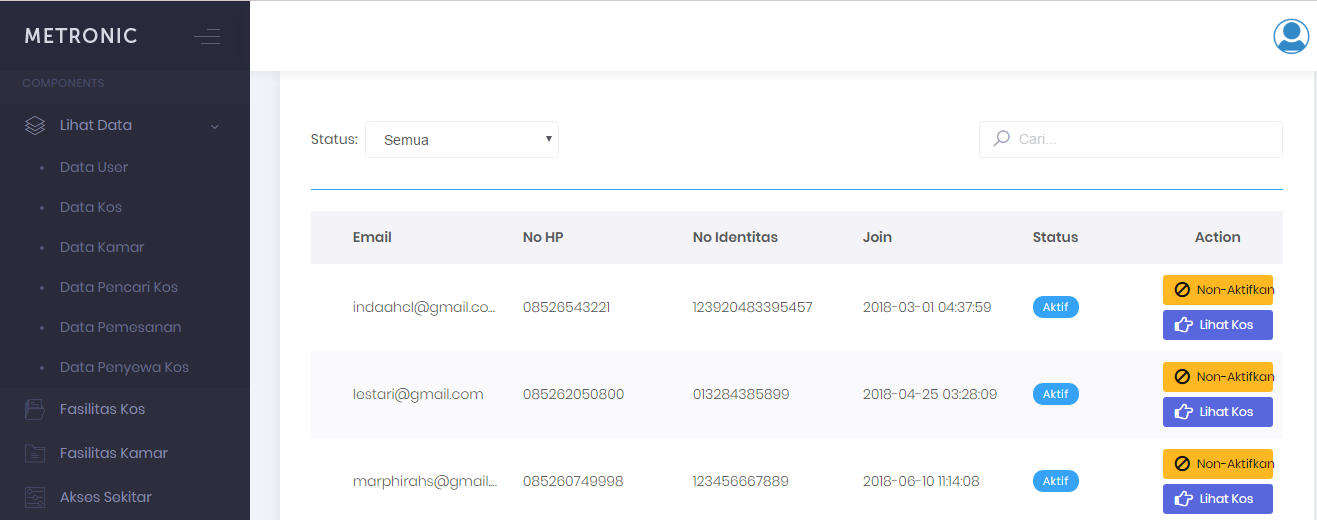
\includegraphics[width=\textwidth]{gambar/a1}
			\caption{Halaman daftar akun}
			\label{webA1}
		\end{figure}
	
	Gambar \ref{webA1} adalah halaman yang memuat daftar pemilik kos yang telah mendaftar pada aplikasi ini. Jika suatu saat terjadi kecurangan atau hal yang dapat menimbulkan kerugian orang lain, maka admin dapat mematikan atau mengnonaktifkan akun pemilik kos.
	
	\begin{figure}[H]
		\centering
		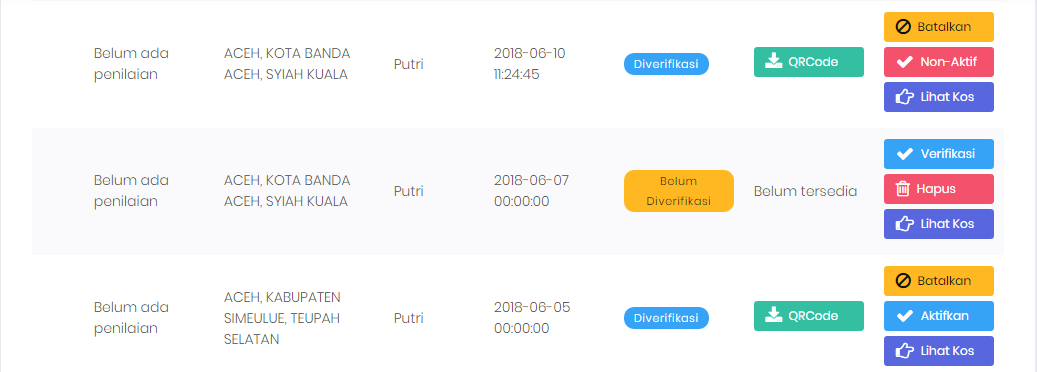
\includegraphics[width=\textwidth]{gambar/a2}
		\caption{Halaman daftar akun}
		\label{webA2}
	\end{figure}
	
	Gambar \ref{webA2} adalah halaman yang memuat daftar kos-kosan yang didaftarkan oleh pemilik kos. Admin dapat memverifikasi kos, membatalkannya dan mengnonaktifkan kos, mengaktifkannya kembali, jika diperlukan.
	\end{enumerate}

		\subsection{Tampilan Halaman Aplikasi Android}
		
		\begin{figure}[H]
			\centering
			
\includegraphics[scale=0.25]{gambar/and/1}
			\caption{\textit{Flash screen} pada aplikasi Android}
			\label{and1}
		\end{figure}
	
		Ketika membuka aplikasi ini maka akan menampilkan \textit{splash screen} selama 3 detik seperti pada gambar \ref{and1}. 
		
		\begin{figure}[H]
			\centering
			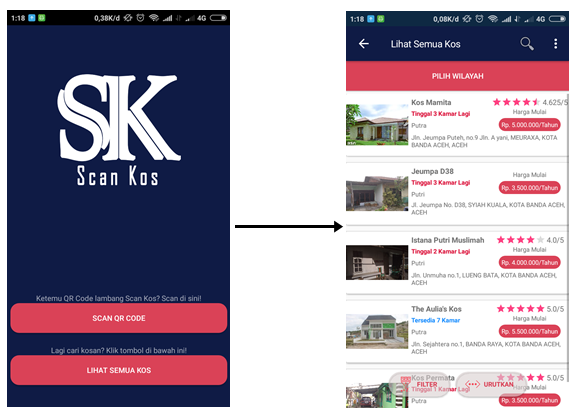
\includegraphics[width=\textwidth]{gambar/and/and1}
			\caption{Halaman awal dan halaman Lihat Semua Kos pada aplikasi Scan Kos Android}
			\label{and2}
		\end{figure}
	
		Gambar \ref{and2} adalah tampilan halaman awal setelah \textit{splash screen }berakhir. Pada halaman awal terdapat dua menu, yaitu Scan QR Code dan Lihat Semua Kos. Jika pengguna menekan tombol Lihat Semua Kos maka akan menampilkan halaman seperti gambar \ref{and2}. Halaman Lihat Semua Kos akan menampilkan semua kos-kosan yang terdaftar pada aplikasi Scan Kos, tetapi hanya kos yang terverifikasi saja yang dapat tampil pada aplikasi Scan Kos. Pengguna dapat memilih kos sesuai kebutuhan, seperti pilih berdasarkan wilayah, \textit{filter}, urutkan berdasarkan harga serta mencari kos dengan kata kunci dari kos-kosan.
		
		\begin{figure}[H]
			\centering
			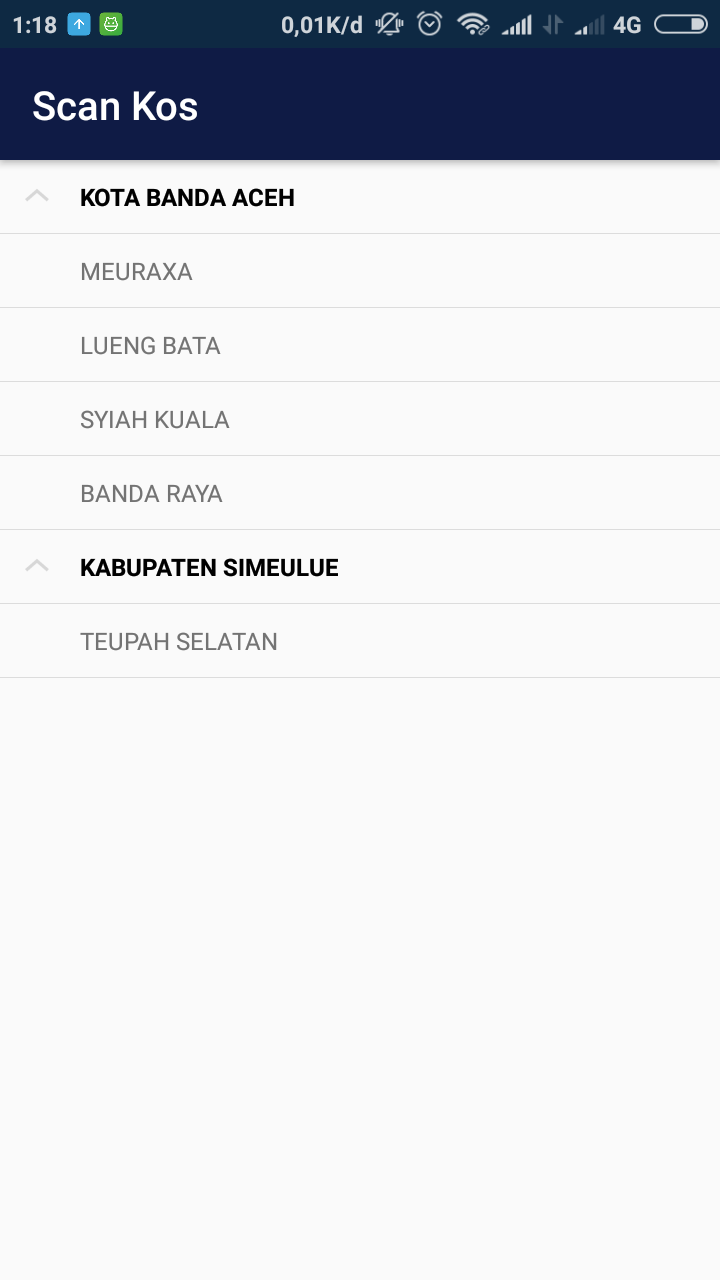
\includegraphics[scale=0.25]{gambar/and/4}
			\caption{Halaman pilih wilayah}
			\label{and3}
		\end{figure}
	
		Gambar \ref{and3} adalah halaman pilih kos berdasarkan wilayah. Wilayah yang tersedia berdasarkan wilayah pada kos-kosan yang terdaftar. Sehingga tidak semua wilayah di Indonesia akan ditampilkan.
		
		\begin{figure}[H]
			\centering
			\includegraphics[scale=0.25]{gambar/and/5}
			\caption{Halaman \textit{filter}}
			\label{and4}
		\end{figure}
	
		Gambar \ref{and4} adalah tampilan halaman \textit{filter}, pengguna dapat memilih kos berdasarkan jenis kos, harga dan fasilitas kos.
		
		\begin{figure}[H]
			\centering
			\includegraphics[scale=0.25]{gambar/and/6}
			\caption{Halaman urutkan kos berdasarkan harga}
			\label{and6}
		\end{figure}
	
		Gambar \ref{and6} adalah halaman untuk mengurutkan kos berdasarkan harga tertinggi atau harga terendah.
		
		\begin{figure}[H]
			\centering
			\includegraphics[width=\textwidth]{gambar/and/and2}
			\caption{Halaman detail kos}
			\label{and7}
		\end{figure}
	
		Gambar \ref{and7} adalah tampilan jika pengguna menekan salah satu kos. Pada halaman detail kos, akan ditampilkan seluruh informasi yang di-\textit{input} oleh pemilik kos. Seperti informasi kontak pemilik kos, jenis kos, jumlah kamar yang disewakan, peta kos, dan penilaian dari penyewa kos.
		
		\begin{figure}[H]
			\centering
			\includegraphics[width=\textwidth]{gambar/and/and3}
			\caption{Halaman detail kamar}
			\label{and8}
		\end{figure}
	
		Pada halaman detail kos, terdapat tab kamar yang menampilkan informasi detail tentang kamar seperti pada gambar \ref{and8}. 
		
		\begin{figure}[H]
			\centering
			\includegraphics[width=\textwidth]{gambar/and/and4}
			\caption{Halaman \textit{login} sebelum dapat memesan kamar}
			\label{and9}
		\end{figure}
	
		Jika pengguna ingin memesan kamar kos, maka pengguna dapat memesan dengan menekan tombol Pesan Kamar. Untuk memesan kamar, pengguna harus \textit{login }terlebih dahulu dengan menggunakan akun Google. Jika sudah \textit{login}, pengguna dapat memesan kamar yang diinginkan. 
		
		\begin{figure}[H]
			\centering
			\includegraphics[scale=0.25]{gambar/and/12}
			\caption{Halaman memilih jangka waktu menyewa kos}
			\label{and10}
		\end{figure}
	
		Gambar \ref{and10} adalah halaman dimana pengguna yang ingin memesan kamar, harus memilih jangka waktu yang diinginkan seperti menyewa kamar per hari, per bulan dan per tahun.
		
		\begin{figure}[H]
			\centering
			\includegraphics[width=\textwidth]{gambar/and/and5}
			\caption{Halaman detail calon penyewa kos}
			\label{and11}
		\end{figure}
		
		Gambar \ref{and11} adalah halaman dimana pengguna harus mengisi data diri untuk dapat memesan kamar kos. Data diri seperti nama, alamat asal, nomor telepon yang dapat dihubungi serta mengupload foto KTP. 
		
		\begin{figure}[H]
			\centering
			\includegraphics[width=\textwidth]{gambar/and/and6}
			\caption{Halaman daftar pemesanan kamar kos}
			\label{and12}
		\end{figure}
		
		Gambar \ref{and12} adalah tampilan ketika pengguna menekan tombol pesan sekarang. Kos yang dipesan akan tampil pada halaman Profil dan Pemesanan di tab Cek Pemesanan. Kamar kos yang dipesan akan masuk ke aplikasi web yang digunakan oleh pemilik kos. Pada tahap ini diharapkan terjadi kontak antara pemilik kos dan calon penyewa kos. Jika pemilik kos dan calon penyewa kos sudah sepakat untuk sewa-menyewa, maka pemilik kos akan menerima calon penyewa tersebut di aplikasi Scan Kos web. Karena sudah disetujui, maka pesanan yang ada di halaman tab Cek Pemesanan akan hilang, dan berpindah ke tab Kos Sekarang. 
		
		\begin{figure}[H]
			\centering
			\includegraphics[scale=0.25]{gambar/and/18}
			\caption{Halaman Kos Sekarang}
			\label{and13}
		\end{figure}
	
		Gambar \ref{and13} adalah halaman tab Kos Sekarang yaitu ketika kamar kos yang dipesan sudah disetujui oleh pemilik kos. Halaman ini akan menampilkan tanggal masuk dan tanggal keluar dari penyewa kos. Selain tab Kos Sekarang, terdapat tab Selesai Kos yaitu halaman yang memuat riwayat kos yang pernah dipesan.
		
		\begin{figure}[H]
			\centering
			\includegraphics[scale=0.25]{gambar/and/17}
			\caption{Halaman Pembatalan Pesanan}
			\label{and14}
		\end{figure}
	
		Gambar \ref{and14} adalah halaman tab Pembatalan Pesanan yaitu pemesanan kamar kos yang dibatalkan oleh calon penyewa kos, pemilik kos dan sistem.
		
		\begin{figure}[H]
			\centering
			\includegraphics[scale=0.25]{gambar/and/19}
			\caption{Halaman Penilaian Kos}
			\label{and15}
		\end{figure}
	
		Sebelumnya pada gambar \ref{and15}, terdapat tombol penilaian kos. Sehingga penyewa dapat memberika penilaian terhadap kamar kos yang telah ia pesan seperti pada gambar \ref{and15}. Hasil dari penilaian dapat dilihat pada gambar \ref{and8}
	
		
	\section{Pengujian Sistem}	
	Tahap terakhir pada perancangan sistem adalah pengujian sistem. Pada aplikasi web, pengujian dilakukan dengan menggunakan pengujian BlackBox sedangkan pada aplikasi Android menggunakan pengujian User Interface (UI) dengan framework Espresso. Kedua pengujian memiliki tujuan yang sama yaitu mengecek apakah sistem sudah berjalan sebagaimana mestinya tanpa error. Setelah pengujian sistem dilakukan, selanjutnya adalah melakukan pengujian kegunaan yang dilakukan oleh pengguna akhir. Pengujian kegunaan yang dimaksud adalah \textit{System Usability Scale} (SUS). 
	
	\subsection{Pengujian pada Aplikasi Android Menggunakan Espresso}
		
		Penulis menggunakan Record Espresso Test yaitu menguji aplikasi tanpa menulis kode. Hal ini dapat memudahkan penulis dalam melakukan pengujian UI. Record Espresso Test tersedia pada Aplikasi Android Studio versi 2.3 keatas. Gambar \ref{espresso} adalah letak Record Espresso Test di Android Studio.
		
		\begin{figure}[H]
			\centering
			\includegraphics[scale=0.6]{gambar/espresso}
			\caption{Halaman Penilaian Kos}
			\label{espresso}
		\end{figure}
		
		Berikut adalah hasil dari pengujian dengan menggunakan Espresso.
		
		\begin{longtable}{ |c|p{5cm}|p{7cm}| }
			\caption{Pengujian UI menggunakan Espresso}
			\label{ujiAndroid} \\
			\hline
			No. &Nama Unit&Hasil Pengujian \\ \hline
			1. &MainActivityTest.java& 
			\begin{minipage}{7cm}
				\smallskip
				\includegraphics[scale=0.6]{gambar/testingAndroid/mainAct}
				\smallskip
			\end{minipage}
			 \\ \hline
			 
			 2. &SemuaKosActivityTest.java& 
			 \begin{minipage}{7cm}
			 	\smallskip
			 	\includegraphics[scale=0.6]{gambar/testingAndroid/semuaAct}
			 	\smallskip
			 \end{minipage}
			 \\ \hline
			 
			 3. &DetailActivityTest.java& 
			 \begin{minipage}{7cm}
			 	\smallskip
			 	\includegraphics[scale=0.6]{gambar/testingAndroid/detailAct}
			 	\smallskip
			 \end{minipage}
			 \\ \hline
			 
			 4. &PesanActivityTest.java& 
			 \begin{minipage}{7cm}
			 	\smallskip
			 	\includegraphics[scale=0.6]{gambar/testingAndroid/pesanAct}
			 	\smallskip
			 \end{minipage}
			 \\ \hline
			 
			 5. &BatalkanPesananActivity-Test.java& 
			 \begin{minipage}{7cm}
			 	\smallskip
			 	\includegraphics[scale=0.6]{gambar/testingAndroid/batalAct}
			 	\smallskip
			 \end{minipage}
			 \\ \hline
			 
			  6. &ProfilActivityTest.java& 
			 \begin{minipage}{7cm}
			 	\smallskip
			 	\includegraphics[scale=0.6]{gambar/testingAndroid/profilAct}
			 	\smallskip
			 \end{minipage}
			 \\ \hline
			 
			 7. &PenilaianActivityTest.java& 
			 \begin{minipage}{7cm}
			 	\smallskip
			 	\includegraphics[scale=0.6]{gambar/testingAndroid/penilaianAct}
			 	\smallskip
			 \end{minipage}
			 \\ \hline
			
		\end{longtable}
		
	Berdasarkan tabel \ref{ujiAndroid}, dari tujuh unit atau kelas yang diuji, semuanya berhasil. Sehingga aplikasi Android sudah berjalan dengan baik dalam segi UI.
	
	\subsection{Pengujian pada Aplikasi Web Menggunakan \textit{Blackbox Testing}}
	
	Kerena tidak ada pengujian UI secara langsung seperti Espresso, maka pengujian aplikasi web menggunakan blackbox testing. Berikut adalah hasil dari pengujian ini.
	
	\begin{longtable}{ |c|p{3cm}|p{3cm}|p{3cm}|p{2cm}|}
		\caption{Pengujian UI menggunakan Espresso}
		\label{ujiWeb} \\
		\hline
		No. & Nama Pengujian & Skenario & Luaran & Hasil Pengujian \\ \hline
		\multirow{4}{*}{1.} & 	\multirow{4}{*}{Daftar akun} & Klik \textit{link} "Silahkan Daftar" & Tampil form yang harus diisi oleh pengguna. & Berhasil \\ \cline{3-5}
		& & Pengguna mengosongkan salah satu \textit{form} & Keluar peringatan bahwa semua \textit{form} wajib diisi & Berhasil \\ \cline{3-5}
		& & Pengguna mendaftarkan akun dengan email yang sama & Keluar peringatan bahwa tidak bisa mendaftarkan akun dengan email yang sama & Berhasil \\ \cline{3-5}
		& & Klik "Daftar" & Pengguna berhasil mendaftar & Berhasil \\ \hline
		
		\multirow{3}{*}{2.} & 	\multirow{4}{*}{\textit{Login} akun} & Pengguna salah masukkan email/password & Keluar peringatan bahwa email/password salah. & Berhasil \\ \cline{3-5}
		& & Pengguna tidak memasukkan salah satu \textit{form} & Keluar peringatan bahwa semua form harus diisi. & Berhasil \\ \cline{3-5}
		& & Klik "Masuk" & Berhasil login dan masuk ke halaman \textit{dashboard} & Berhasil \\ \hline
		
		\multirow{2}{*}{3.} & 	\multirow{2}{*}{Tambah data kos} & Pengguna mengosongkan salah satu form & Keluar peringatan bahwa semua form wajib diisi. & Berhasil \\ \cline{3-5}
		&& Klik "Simpan" & Data kos berhasil disimpan & Berhasil \\ \hline
		
		\multirow{2}{*}{4.} & 	\multirow{2}{*}{Tambah data kamar} & Pengguna mengosongkan salah satu form & Keluar peringatan bahwa semua form wajib diisi. & Berhasil \\ \cline{3-5}
		&& Klik "Simpan" & Data kamar berhasil disimpan & Berhasil \\ \hline
		
		\multirow{4}{*}{4.} & 	\multirow{4}{*}{Lihat data kos} & Klik hapus & Keluar peringatan seperti "Apakah Anda yakin akan menghapus kos ini?" Jika ya, maka kos berhasil dihapus. Jika tidak, kos tidak dihapus. & Berhasil \\ \cline{3-5}
		&& Klik Lihat Detail & Menampilkan halaman informasi kos yang lebih detail serta kamar & Berhasil \\ \cline{3-5}
		&& Lihat Penilaian & Menampilkan halaman penilaian yang diberikan oleh penyewa kos & Berhasil \\ \cline{3-5}
		&& Download QR Code & Menampilkan gambar QR Code dari kos tersebut & Berhasil \\ \hline
		
		5. & Lihat data kamar & 
		Klik Penuh& Jumlah kamar yang ada sama dengan jumlah kamar yang terisi sehingga kamar kos menjadi tidak aktif & Berhasil \\ \hline
		
		\multirow{5}{*}{6.} & 	\multirow{5}{*}{Lihat data pemesanan} & Klik Lihat CP (Calon Penyewa) & Menampilkan data calon penyewa beserta foto KTP & Berhasil \\ \cline{3-5}
		&& Klik Terima & Menampilkan form yang harus diisi oleh pemilik kos & Berhasil \\ \cline{3-5}
		&& Mengosongkan salah satu form & Keluar peringatan bahwa form harus diisi semua & Berhasil \\ \cline{3-5}
		&& Klik Simpan & Data berhasil disimpan dan penyewa kos bertambah & Berhasil \\ \cline{3-5}
		&& Klik Tolak & Berhasil menolak pesanan & Berhasil \\ \hline
		
		\multirow{2}{*}{7.} & 	\multirow{2}{*}{Lihat data penyewa} & Klik edit & Menampilkan form untuk mengubah tanggal keluar atau keterangan & Berhasil \\ \cline{3-5}
		&& Klik Simpan & Data berhasil diubah & Berhasil \\ \hline
		
	\end{longtable}

	Berdasarkan tabel \ref{ujiWeb} seluruh pengujian yang telah dilakukan berhasil sehingga aplikasi web sudah berjalan dengan baik. 
	
	\subsection{Pengujian Kegunaan dengan metode \textit{System Usability Scale }(SUS)}
	
	Setelah melakukan pengujian sistem, selanjutnya aplikasi akan diuji dengan pengujian SUS. SUS memiliki kuesioner
	yang terdiri dari 10 pertanyaan. Pertanyaan dari SUS dapat dilihat pada tabel \ref{kuesioner}.
	
	Tahapan yang dilakukan dalam pengujian SUS adalah sebagai berikut:
	
	\begin{enumerate}[a.]
		\item Menentukan skenario pengujian, yaitu menyusun tugas-tugas yang akan dilakukan oleh pengguna. Berikut adalah skenario yang akan dilakukan oleh responden kelompok pengguna pemilik kos untuk menggunakan aplikasi Scan Kos berbasis Web.
		
		\begin{longtable}{ |c|p{5cm}|p{7cm}| }
			\caption{Daftar Tugas Responden Pemilik Kos}
			\label{skenarioPK} \\
			\hline
			No. & Tugas & Deskripsi \\
			\hline
			1. & Membuka aplikasi &  \\
			\hline
			2.  & Klik link "Silahkan Daftar" & Jika belum memiiki akun, maka pemilik kos harus mendaftarkan diri\\
			\hline
			3. & Mengisi data diri & Untuk mengisi data diri\\
			\hline
			4. & Klik tombol Daftar & Untuk mendapatkan akun dan terdaftar diaplikasi Scan Kos web\\
			\hline
			5. & Klik Tambah Data Kos & Pemilik kos dapat menambahkan data kos\\
			\hline
			6. & Mengisi data kos & Untuk mengisi data kos \\
			\hline
			7. & Klik Simpan & Untuk menyimpan data kos \\
			\hline
			8. & Klik Tambah Data Kamar & Setelah data kos, pemilik kos dapat menambahkan data kamar\\
			\hline
			9. & Mengisi data kamar & Untuk mengisi data kamar \\
			\hline
			10. & Klik Simpan & Untuk menyimpan data kamar \\
			\hline
			11. & Klik Data Kos & Untuk melihat data kos yang sudah di-input \\
			\hline
			12. & Klik lihat detail & Untuk melihat detail dari kos dan kamar \\
			\hline
			13. & Klik lihat penilaian di tab kos & Untuk kos yang pernah dipesan dan penyewa memberi penilaian maka pemilik kos dapat melihat penilaian tersebut \\
			\hline
			14. & Klik tab kamar & Untuk melihat detail data kamar \\
			\hline
			15. & Klik \textit{download QR Code} di halaman data kos & Untuk kos yang sudah diverifikasi, maka dapat men\textit{download QR Code} yg berisi informasi kos milik akun \\
			\hline
			16. & Klik Data Kamar & Melihat rekap seluruh data kamar \\
			\hline
			17. & Klik tombol Penuh & Untuk kamar yang sudah penuh (tidak disewa lagi) \\
			\hline
			18. & Klik Data Pemesanan & Melihat para calon penyewa memesan kamar kos \\
			\hline
			19. & Klik Lihat CP (calon penyewa) & Melihat data dari calon penyewa \\
			\hline
			20. & Klik terima di halaman data pemesanan & Untuk menyetujui penyewaan \\
			\hline
			21. & Klik Data Penyewa & Melihat orang-orang yang telah menyewa kos miliknya \\
			\hline
			22. & \textit{Logout} & Keluar dari aplikasi \\
			\hline
		\end{longtable}
		
		Berikut adalah skenario yang akan dilakukan oleh responden kelompok pengguna pencari kos untuk menggunakan aplikasi Scan Kos berbasis Android.
		
		\begin{longtable}{ |c|p{5cm}|p{7cm}| }
			\caption{Daftar Tugas Responden Pemilik Kos}
			\label{skenarioPencari} \\
			\hline No. & Tugas & Deskripsi \\
			\hline
			1. & Membuka aplikasi & - \\
			\hline
			2. & Klik tombol Lihat Semua Kos & Untuk melihat semua daftar kos. Setelah diklik, maka akan menampilkan halaman yang memuat semua kos-kosan. \\
			\hline
			3. & Klik tombol Pilih Wilayah & Mencari kos berdasarkan daerah tertentu. \\
			\hline
			4. & Klik tombol Filter & Memilih kos sesuai keinginan. \\
			\hline
			5. & Klik tombol Urutkan & Memilih kos berdasarkan urutan harga. \\
			\hline
			6. & Klik icon Search & Mencari kos berdasarkan nama. \\
			\hline
			7. & Klik salah satu kos & Melihat detail informasi kos (dapat di \textit{scroll}). \\
			\hline
			8. & Klik tab Kamar & Melihat detail kamar. \\
			\hline
			9. & Klik Pesan Kamar & Memesan kamar yang diinginkan. \\
			\hline
			10. & Login	& Sebelum pesan, \textit{login }dahulu. \textit{Login} menggunakan akun Google. \\
			\hline
			11. & Pilih Jangka Waktu & Jangka waktu yang diinginkan untuk menyewa kos \\
			\hline
			12. & Klik Isi Detail… & Untuk mengisi data diri \\
			\hline
			13. & Masukkan data diri & Data akan dilihat oleh pemilik kos \\
			\hline
			14. & Klik Simpan & Simpan data \\
			\hline
			15. & Klik Pesan Sekarang & Pesanan akan diproses \\
			\hline
			16. & Klik Tab Kos Sekarang & Melihat data pemesanan kos yang sudah disetujui \\
			\hline
			17. & Klik Beri Penilaian & Untuk melakukan \textit{rating} dan komentar \\
			\hline
			18. & Masukkan penilaian & Penilaian untuk kamar/kos yang ditempati \\
			\hline
			19. & Klik Submit & Penilaian disimpan \\
			\hline
			20. & Klik Lihat Kos & Melihat \textit{rating }yang sudah di\textit{input} \\
			\hline
			21. & Kembali ke tugas nomor 7-15 & - \\
			\hline
			22. & Klik Data Pemesanan Kos di Tab Cek Pemesanan & Untuk melihat detail dari pesanan seperti data diri dan status pemesanan. \\
			\hline
			23. & Klik Batalkan Pemesanan & Untuk membatalkan pesanan kos. \\ 
			\hline
			24. & Klik Tab Pembatalan Pesanan & Melihat daftar riwayat pembatalan pemesanan kos \\
			\hline
			25. & Klik Scan QR Code	& Mendapatkan informasi suatu kos \\
			\hline
			26. & \textit{Logout} & Keluar dari aplikasi \\ 
			\hline
		\end{longtable}
		\item Pemilihan responden dan jumlah responden. Responden yang dipilih adalah kelompok pengguna yang akan menggunakan aplikasi Scan Kos. Sehingga respondennya terdiri dari pencari kos (penyewa kos) dan pemilik kos. Masing-masing kelompok pengguna berjumlah 30 responden. Rentang umur responden pemilik kos dari umur 33 tahun sampai 54 tahun sedangkan responden pencari kos dari 18 tahun sampai 23 tahun. Responden pemilik kos didapat dengan cara mengunjungi kos-kosan yang berada sekitaran Banda Aceh. Sedangkan responden pencari kos didapat dengan cara menjumpai mahasiswa baru yang sedang melakukan pendaftaran ulang di Unsyiah dan juga dengan cara mengunjungi kos-kosan.
		\item Pengujian aplikasi oleh responden. Responden akan melakukan skenario yang telah dibuat.
		\item Pengisian kuisioner oleh responden. Responden akan mengisi kuisioner SUS yang diberikan seperti pada tabel \ref{sus}.
		
	\end{enumerate}
	
	Setelah tahapan pengujian SUS dilakukan, selanjutnya adalah menghitung nilai SUS setiap responden. Cara menghitung nilai SUS adalah sebagai berikut:
	\begin{enumerate}[a.]
		\item  Untuk pernyataan ganjil: skala yang diberikan responden dikurangi satu.
		\item Untuk pernyataan genap: lima dikurangi skala yang diberikan responden.
		\item Skala Sangat Tidak Setuju sampai Sangat Setuju bernilai 0 sampai 4.
		\item Jumlahkan skala responden yang telah dikonversi dan kalikan jumlahnya dengan 2,5. Ini mengkonversi rentang nilai menjadi antara 0-100. Nilai tersebut bukanlah persen.
	\end{enumerate} 

	Hasil perhitungan nilai SUS pada responden pemilik kos dan pencari kos dapat dilihat pada Lampiran 1. Dari 30 responden pemilik kos, jumlah nilai SUS adalah 72,5 dan dari 30 responden pemilik kos, jumlah nilai SUS adalah 80,6. Selanjutnya menentukan \textit{grade} hasil perhitungan SUS dengan melihat sisi tingkat penerimaan pengguna, \textit{grade }skala dan \textit{adjective ratings}. Penentuan grade tersebut dapat dilihat pada gambar \ref{susScore}.
	
	\begin{figure}[H]
		\centering
		\includegraphics[width=\textwidth]{gambar/susscore}
		\caption{SUS Score}
		\label{susScore}
	\end{figure}

	Hasil penilaian terhadap aplikasi Scan Kos adalah sebagai berikut:
	\begin{enumerate}[a.]
		\item Pemilik Kos
		
		Hasil perhitungan nilai SUS pada responden pemilik kos adalah 72,5. Nilai ini akan dibandingkan dengan SUS Score pada gambar \ref{susScore}. Hasilnya adalah:
		\begin{enumerate}[-]
			\item Pada Acceptability Ranges masuk pada kategori Acceptable
			\item Pada Grade Scale masuk pada kategori C
			\item Pada Adjective Ratings masuk pada kategori Good
		\end{enumerate}
		\item Pencari Kos
		
		Hasil perhitungan nilai SUS pada responden pencari kos adalah 80,6. Nilai ini akan dibandingkan dengan SUS Score pada gambar \ref{susScore}. Hasilnya adalah:
		\begin{enumerate}[-]
			\item Pada Acceptability Ranges masuk pada kategori Acceptable
			\item Pada Grade Scale masuk pada kategori B
			\item Pada Adjective Ratings masuk pada kategori Excellent
		\end{enumerate}
	\end{enumerate}

	Hasil dari kedua kelompok responden menunjukkan bahwa Aplikasi Scan Kos berbasis web maupun Android masuk ke dalam kategori \textit{Acceptable }atau dapat diterima oleh pengguna akhir. 
	
% Baris ini digunakan untuk membantu dalam melakukan sitasi.
% Karena diapit dengan comment, maka baris ini akan diabaikan
% oleh compiler LaTeX.
\begin{comment}
\bibliography{daftar-pustaka}
\end{comment}